\documentclass[
      12pt,
        ]{article}






% --- type and typeface? -----------------------

% input
\usepackage[utf8]{inputenc}

% typography
\usepackage{microtype}


\usepackage[T1]{fontenc}


% text block
\usepackage{setspace}
\usepackage[ 
              left = 1in,top = 1in,right = 1in,bottom = 1in 
            ]{geometry}

\usepackage{enumitem}
  \setlist{noitemsep}



% decimal numbering for appendix figs and tabs


% Deletes section counters
% \setcounter{secnumdepth}{0}







  \usepackage{longtable, booktabs}









  \usepackage{natbib}
  \bibliographystyle{/Users/devin/dissertation/assets/apsr.bst}
  % protect underscores in most circumstances
  \usepackage[strings]{underscore} 


% 

% \newtheorem{hypothesis}{Hypothesis}

\makeatletter
  \@ifpackageloaded{hyperref}{}{%
    \ifxetex
      % page size defined by xetex
      % unicode breaks when used with xetex
      \PassOptionsToPackage{hyphens}{url}\usepackage[setpagesize = false, 
                                                     unicode = false, 
                                                     xetex]{hyperref}
    \else
      \PassOptionsToPackage{hyphens}{url}\usepackage[unicode = true]{hyperref}
    \fi
  }

  \@ifpackageloaded{color}{
    \PassOptionsToPackage{usenames,dvipsnames}{color}
  }{
    \usepackage[usenames,dvipsnames]{color}
  }
\makeatother

\hypersetup{breaklinks = true,
            bookmarks = true,
            pdfauthor = {Devin Judge-Lord ()},
             pdfkeywords  =  {},  
            pdftitle = {Why Do Agencies (Sometimes) Get So Much Mail?: Public Pressure Campaigns and Bureaucratic Policymaking},
            colorlinks = true,
            citecolor = black,
            urlcolor = blue,
            linkcolor = magenta,
            pdfborder = {0 0 0}}

% \urlstyle{same}  % don't use monospace font for urls


% set default figure placement to htbp
\makeatletter
  \def\fps@figure{hbtp}
\makeatother


% optional footnotes as endnotes


% ----- Pandoc wants this tightlist command ----------
\providecommand{\tightlist}{
  \setlength{\itemsep}{0pt}
  \setlength{\parskip}{0pt}
}





% --- title & section styles -----------------------


% title, author, date
  \title{Why Do Agencies (Sometimes) Get So Much Mail?: 
           \\ Public Pressure Campaigns and Bureaucratic Policymaking}
 

  \author{ % author, option footnote, optional affiliation
            Devin Judge-Lord\footnote{University of Wisconsin-Madison, \href{mailto:judgelord@wisc.edu}{\nolinkurl{judgelord@wisc.edu}}. Slides and the most recent draft are available at \url{https://judgelord.github.io/research/whymail}} 
            }

% auto-format date?
  \date{2020-08-13}


% abstract
\usepackage{abstract}
  \renewcommand{\abstractname}{}    % clear the title
  \renewcommand{\absnamepos}{empty} % originally center

  \newcommand*{\authorfont}{\sffamily\selectfont}


% section titles
\usepackage[small, bf, sc]{titlesec}
  % \titleformat*{\subsection}{\itshape}
  \titleformat*{\subsubsection}{\itshape} 
  \titleformat*{\paragraph}{\itshape} 
  \titleformat*{\subparagraph}{\itshape}



%\usepackage{float}
%\floatstyle{plaintop}
%\restylefloat{table}
\usepackage{floatrow}
\floatsetup[figure]{capposition=top}
\floatsetup[table]{capposition=top}
\usepackage{multirow}
\usepackage{rotating} 
\usepackage{caption}






















\begin{document}
 

% --- PAGE: title and abstract -----------------------

  \maketitle

% \pagenumbering{gobble}
  \pagenumbering{gobble}



  \begin{abstract}
    \noindent THIS DRAFT WAS PREPARED FOR THE 2020 AMERICAN POLITICAL ECONOMY WORKSHOP. SLIDES AND THE MOST RECENT DRAFT ARE \href{https://judgelord.github.io/research/whymail/}{HERE}

\bigskip

I examine who participates in public pressure campaigns and why. Scholars of bureaucratic policymaking have focused on the sophisticated lobbying efforts of powerful interest groups. Yet agencies occasionally receive thousands or even millions of comments from ordinary people. How, if at all, should scholars incorporate mass participation into models of bureaucratic policymaking? Are public pressure campaigns, like other lobbying tactics, primarily used by well-resourced groups to create an impression of public support? Or are they better understood as conflict expansion tactics used by less-resourced groups? To answer these questions, I collect and analyze millions of public comments on draft agency rules. Using text analysis methods underlying plagiarism detection, I match individual public comments to pressure-group campaigns. I find that most public comments are mobilized by a few public interest organizations. Over 80\% of the 48 million comments on proposed rules posted to regulations.gov were mobilized by just 100 organizations, 87 of which lobby in coalitions with each other. Contrary to other forms of lobbying, I find that mass comment campaigns are almost always a conflict expansion tactic, rather than well-resourced groups creating an impression of public support. Contrary to other forms of political participation, I find no evidence of negativity bias in public comments. Indeed, from 2005 to 2017, most comments supported proposed rules. This is because public comments tend to support Democratic policies and oppose Republican policies, reflecting the asymmetry in mobilizing groups. 

    

  \end{abstract}



% --- PAGE: contents -----------------------





% --- PAGE: body -----------------------


  \newpage
  \pagenumbering{arabic}

\noindent 
 
   
   
\textbf{Note to reader:} This dissertation chapter develops concepts and measures of public engagement in rulemaking that I apply in chapters 3 and 4. The methods are under construction, and the empirical claims are tentative.

This project aims to better understand the role of ordinary people in bureaucratic policymaking.
I develop theories of why mass engagement occurs and how it may affect policy. To assess these theories, I tackle three related empirical questions: (1) Why does it occur?; (2) How does it affect the oversight behaviors of agencies' political principals?; and
(3) Does mass engagement in bureaucratic policymaking affect policy?

\textbf{Chapter 1 situates agency rulemaking in the context of American politics.} I show that rulemaking is a major site of policymaking and political conflict.

\textbf{Chapter 2 explains why agencies (occasionally) get so much mail.}
The literature suggests two possible explanations for variation in mass engagement; groups may leverage public support as a lobbying resource (``grassroots'' mobilization) or groups with more resources may leverage those resources into an impression of public support (sometimes called ``astroturf'').
I find that public interest campaigns explain variation in mass engagement. Unlike other forms of lobbying, it is not primarily driven by interests with the largest financial stakes and resources.
Because the vast majority of comments are inspired by interest-group campaigns, finding their cause requires a method to link comments to the lobbying coalitions that mobilized them. To link individual comments to the more sophisticated lobbying efforts they support, I use text reuse and clustering methods to capture formal and informal coalitions.

\textbf{Chapter 3 asks whether public pressure campaigns affect political oversight.} The political information signaled by mass engagement may serve as ``fire alarms,'' altering principals to oversight opportunities or ``warning signs'' altering them to political risks.
When a coalition mobilizes successfully,
elected officials ought to be more likely to engage on their behalf and less likely to engage against them.
To assess these hypotheses, I count the number of times Members of Congress engage the agency before, during, and after comment periods on rules where lobbying organizations did and did not go public. I then use text analysis to compare legislators' sentiments and rhetoric to that used by each coalition.

\textbf{Chapter 4 asks whether public pressure campaigns affect rulemaking and rules.}
I theorize that the effects of political information on policy depend on the extent to which the strategic environment allows change and how political information is processed, both directly within agencies and indirectly through other actors (e.g., Members of Congress) whose appraisals matter to bureaucrats.
The main dependent variable is change in the rule text.
I systematically identify changes between draft and final rules, parse these differences to identify meaningful policy changes, and compare them to demands raised in comments to measure which coalition got their desired outcomes.

\textbf{Chapter 5 presents a case study of the environmental justice movement.} I identify all rules where ``environmental justice'' is raised in the comments to assess agency responses both quantitatively and qualitatively. In preliminary analysis, I find that responsiveness to environmental justice activist comments varies in predictable ways across agencies, but I find no evidence that the total number of comments affects rules.

\textbf{Chapter 6} concludes with remarks on the study of bureaucratic policymaking and policy recommendations to better account for the fact that public pressure campaigns and the bursts of civic engagement they mobilize will be an enduring feature of the policy process.

\hypertarget{intro}{%
\section{Introduction}\label{intro}}

\onehalfspacing

With the rise of the administrative state, U.S. federal agencies have
become a major site of policymaking and political conflict. By some
estimates, upward of 90\% of legally binding U.S. federal policy is now
written by agencies. Agency rules are revised much more frequently than
statutory law \citep{Wagner2017}. In the years or decades between
legislative enactments, federal agencies make legally-binding rules
interpreting and reinterpreting old statutes to address emerging issues
and priorities. Examples are striking: Many effects of the Dodd-Frank Wall
Street Reform and Consumer Protection Act were largely unknown until the
specific regulations were written, and it continues to change as these
rules are revised. Congress authorizes billions in grants, subsidies, and
leases for public lands, but who gets them depends on agency policy. In
the decades since the last major environmental legislation, agencies
have written thousands of pages of new environmental regulations and
thousands more changing tack under each new administration. These
revisions significantly shape lives and fortunes. For example, in 2006,
citing the authority of statutes last amended in the 1950s, the Justice
Department's Bureau of Prisons proposed a rule restricting eligibility
for parole. In 2016, the Bureau withdrew this rule and announced it
would require fewer contracts with prison companies,
precipitating a 50\% loss of industry stock value. Six months later, a
new administration announced these policies would again be reversed,
leading to a 130\% increase in industry stock value. Agency rulemaking
matters.

Less clear, however, is how the new centrality of agency rulemaking fits
with democracy. In addition to the bureaucracy's complex relationships with
the president and Congress, agencies have complex and poorly understood
relationships with the public and advocacy groups. Relationships with
constituent groups may even provide agencies with a degree of ``autonomy'' from their official principals \citep{Carpenter2001}.

Participatory processes like public comment periods, where government
agencies must solicit public input on draft policies, are said to provide political oversight opportunities \citep{Balla1998, Mccubbins1984}, democratic legitimacy \citep{Croley2003, Rosenbloom2003}, and new technical information \citep{Yackee2006JPART, Nelson2012}. While recent scholarship on agency policymaking has shed light on sophisticated lobbying by businesses, we know surprisingly little about the vast majority of public comments, which are submitted by ordinary people as part of public pressure campaigns.\footnote{
  As I show below, most comments submitted to
  regulations.gov are part of organized campaigns, more akin to petition signatures than ``deliberative'' participation or sophisticated lobbying. Indeed, approximately 40 million out of
  50 million (80\%) of these public comments mobilized by just 100
  advocacy organizations.}
Activists frequently target agency policymaking with letter-writing campaigns, petitions, protests,
and mobilizing people to attend hearings, all classic examples of ``civic engagement'' \citep{Verba1987}. Yet civic engagement remains poorly understood in the context of bureaucratic policymaking.
While practitioners and administrative law scholars have long pondered
what to make of mass commenting, political scientists have had
surprisingly little to say about this kind of civic participation.

\hypertarget{the-contentious-politics-that-inspire-the-majority-of-public-comments-have-no-place-in-leading-models-of-bureaucratic-policymaking-and-have-largely-been-ignored-by-political-scientists.}{%
\paragraph{The contentious politics that inspire the majority of public comments have no place in leading models of bureaucratic policymaking and have largely been ignored by political scientists.}\label{the-contentious-politics-that-inspire-the-majority-of-public-comments-have-no-place-in-leading-models-of-bureaucratic-policymaking-and-have-largely-been-ignored-by-political-scientists.}}

Foundational scholarship on rulemaking \citep[\citet{Furlong1997}, \citet{Furlong1998}, \citet{Kerwin2011}]{Furlong2005} focuses on interest group lobbying. Theoretical models focus on how agencies learn about policy problems, negotiate or avoid accountability to various principals, or balance interest-group demands.\footnote{On learning, see \citet{Kerwin2011} and empirical studies by \citet{Yackee2012},
  \citet{Cook2017}, \citet{Gordon2018}, and \citet{Walters2019}. See \citet{Gailmard2017} and
  \citet{Libgober2018} for information-based models where comments reveal information to the agency.
  On accountability to elected officials, see \citet{Furlong1997}, \citet{Nou2016},
  \citet{Potter2016}, \citet{Woods2018}, and \citet{Yackee2009RegGov}.
  \citet{Potter2014dis} develops a signaling model where agencies propose and principals veto rules depending, in part, on their beliefs about interest group preferences.
  On interest-group balancing, see \citet{Yackee2006JOP}, \citet{Yackee2006JPART},
  and \citet{Kerwin2011}. A key assumption of Libgober's (2018) model is that
  bureaucrats have a distribution of preferences over interest group
  positions, about which they are uncertain unless groups reveal their
  preferences through commenting.}

\hypertarget{most-scholars-are-skeptical-that-ordinary-people-can-affect-rulemaking.}{%
\paragraph{Most scholars are skeptical that ordinary people can affect rulemaking.}\label{most-scholars-are-skeptical-that-ordinary-people-can-affect-rulemaking.}}

To the extent that scholars address the input of ordinary people at all, both
existing theory and empirical scholarship suggest skepticism that it
matters. (By ``ordinary'' people, I simply mean people who are not
professional policy-influencers.)
Empirical scholarship finds that economic elites and business groups
dominate American politics in general \citep[\citet{Soss2007}, Hertel-Fernandez2019, \citet{Hacker2003}, \citet{Gilens2014}]{Jacobs2005} and rulemaking in
particular. While some are optimistic that requirements for agencies to
solicit and respond to public comments on proposed rules allow ``civil
society'' to provide public oversight \citep{Michaels2015, Metzger2010}, most
studies find that participants in rulemaking often represent elites and
business interests \citep[LibgoberCarpenter2018]{Seifter2016UCLA, Crow2015, Wagner2011, West2009, Yackee2006JOP, Yackee2006JPART, Golden1998, Haeder2015, Cook2017}.

Scholars are thus skeptical about rulemaking as a venue for collective action. As a result, public pressure campaigns are dismissed as epiphenomenal to bargaining with political principals
or interest groups. Indeed, almost all empirical studies of rulemaking
discard unsophisticated comments from ordinary people, as evident from a
comprehensive review of scholarship on ``The Politics of Rulemaking'' by
\citet{Yackee2019}, who finds skepticism about citizen comments, but no studies
analyzing public pressure campaigns as a lobbying tactic:

\begin{quote}
``\citet{Kerwin2011} point out that a citizen must know not only that a regulation is being formulated but also how and when to participate. This is a high bar for most Americans. Second, to be influential during rulemaking, commenters may require resources and technical expertise. As \citet{Epstein2014} suggest, agency rule-writers---who are often chosen because of their technical or policy-specific expertise---privilege the type of data-driven arguments and reasoning
that are not common to citizen comments.'' (p.~10)
\end{quote}

For any particular lay commenter, this conclusion seems inescapable; individuals acting alone are unlikely to affect policy. As Hacker and Pierson (Forthcoming) observe,

\begin{quote}
``{[}The United States'{]} institutional terrain advantages political actors with the capacity to work across multiple venues, over extended periods, and in a political environment where coordinated government action is difficult, and strategies of evasion and exit from regulatory constraints are often successful. These capacities are characteristic of organized groups, not individual voters.''
\end{quote}

But groups occasionally mobilize a large number of people, usually behind a more sophisticated lobbying effort. Without a systematic understanding of the scale and impact of public participation--\emph{group-mediated} participation--in rulemaking, it is impossible to answer normative questions about how participatory processes like public comment periods may enhance or undermine various democratic ideals.

Scholars' neglect of public pressure campaigns is surprising given that most people are only
aware of agency rulemaking when it is the target of a high-profile mass
mobilization campaign.\footnote{Some of the most contentious recent public controversies involve
  bureaucratic policymaking. For example, along with 50 thousand
  protesters in Washington D.C., the State Department Received 1.2
  million comments on the Environmental Impact Statement for the
  Keystone Pipeline. Similarly, along with the thousands of protesters
  supporting the Standing Rock Sioux protest to the Dakota Access
  Pipeline, the Army Corps of Engineers received hundreds of thousands
  of comments. Alongside protest actions that included shutting down
  many websites, the Federal Communications Commission's open internet
  rule received 22 million comments. While some of these comments
  appear to be fake, the scale of public engagement is remarkable
  given how little attention political scientists have paid to it.
  Fake public comments also raise the question of why an organization
  would bother to generate fake public input if it did not matter, as
  its omission from theories of bureaucratic policymaking would seem
  to imply.} While most rules receive little attention,
the ease of online mobilizing and commenting has, like other forms of
participation \citep{Boulianne2018}, created exponential increases in the
number of rules in which thousands and even millions of people engage
(see Figure \ref{fig:comments-per-year}; note that comments per rule are on a
logarithmic scale).\footnote{Proposed rules that have attracted the most public attention have
  been published by the Federal Communications Commission (FCC,
  omitted from this plot), the Environmental Protection Agency (EPA),
  the Department of Interior (DOI), the Bureau of Ocean Energy
  Management (BOEM), the Consumer Financial Protection Bureau (CFPB),
  and Fish and Wildlife Service (FWS).} Occasionally, a large number of people are
paying attention.

The general failure to explain or account for public pressure campaigns in models of bureaucratic policymaking is also striking in light of how agencies advertise public
comment periods as an opportunity for a voice in government
decisions.\footnote{I focus on public comments in rulemaking, but the theories and
  methods here may also apply to other kinds of political engagement
  such as through social media or protests as well as to other
  political decisions, including state-level rulemaking. Social media
  engagement may be especially important if agencies implement the
  recommendations of \citet{ACUS2018} that ``Agencies should consider using
  social media before or in connection with direct final rulemaking to
  quickly identify whether there are significant or meaningful
  objections'' (p.~34).} Big red letters across the top of the Regulations.gov
homepage solicit visitors to ``Make a difference. Submit your comments
and let your voice be heard'' and ``Participate today!'' (Figure \ref{fig:regsgov}. A blue ``Comment Now!'' button accompanies a short description of each draft
policy and pending agency action.
Public comment periods on proposed agency
rules is described as ``an important part of democracy'' (WSJ 2017),
``often held out as the purest example of participatory democracy in
actual American governance'' \citep{Herz2016}. \citet{Rossi1997} finds that ``courts, Congress, and scholars have elevated participation in rulemaking to
a sacrosanct status\ldots greater participation is generally viewed as
contributing to democracy.''

\begin{figure}

{\centering 
\includegraphics[width=6.5in]{../Figs/regulations-header} 

}

\caption{Regulations.gov Solicits Public Comments on Draft Agency Rules}\label{fig:regsgov}
\end{figure}

\begin{figure}

{\centering 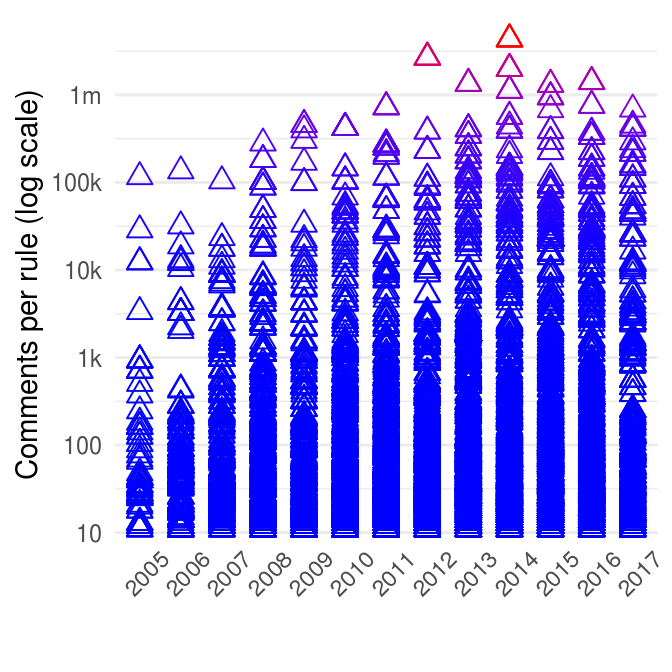
\includegraphics[height=0.25\textheight]{/Users/devin/dissertation/Figs/rules-comments-per-year-1} 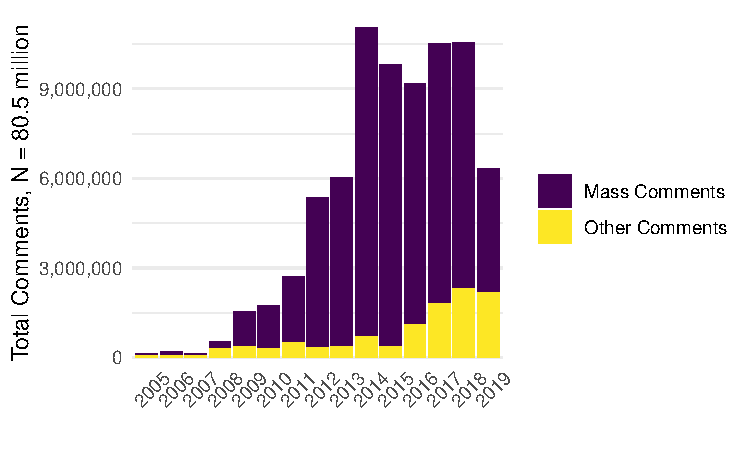
\includegraphics[height=0.25\textheight]{/Users/devin/dissertation/Figs/comments-mass-vs-unique} 

}

\caption{Comments per Proposed Rule and Total Comments per Year}\label{fig:comments-per-year}
\end{figure}

While ``ordinary'' members of the public may occasionally provide novel
and useful technical information to expert bureaucrats, such
sophisticated means of influencing policy are out of reach for the vast
majority of people. Thus, to investigate the potential role of ordinary
people in bureaucratic politics I look elsewhere---not because ordinary
people never provide novel and useful technical information, but because
this is not how most people attempt to influence policy, nor, I argue,
how we should expect ordinary people to have influence.

Most public comments are, in fact, of the type suggested by the
solicitations on Regulations.gov---ordinary people voicing opinions on a proposed policy. They do not provide useful technical information or
suggest specific edits to policy texts like the interest group comments
that have thus far captured the attention of political scientists. If
they add information to rulemaking, it is a different, more political
flavor of information. Indeed as Figure
\ref{fig:comments-per-year} shows, every year since 2008, most people who
comment on draft regulations have done so as a result of a public pressure campaign.\footnote{At least for agencies participating in regulations.gov. See
  sections
  \ref{whyMail-methods} and
  \ref{whyMail-results} for my definition and methods for identifying mass comments.} Public engagement in rulemaking is highly
clustered on a few rules made salient by these campaigns. It is
plausible that at least some of the time, such campaigns aim to
influence policy. It is also plausible that thousands of people engaging
may alter the politics of these policy processes, but this hypothesis
remains untested. Indeed, we have much to understand about the causes
and effects of these campaigns before we are in a position to ask if
they are a mechanism for groups to influence policy. Most critically, we
must understand who mobilizes and why.

The kind of politics created by mass engagement has a few notable
features. It is contentious; most ordinary people are not engaging in
deliberation; they are simply making demands. Importantly, however,
processes like public comment periods channel contentious demands into
institutionalized policy processes rather than undermining them. In
short, the politics of rulemaking created by public pressure campaigns is much
more contentious than most rulemakings, but also much more
institutionalized than most contentious politics. Mass engagement in
rulemaking thus presents a novel context to examine the consequences of
broader public participation in typically insider-dominated policymaking and how
public pressure may condition how political decisions are made.

Public pressure campaigns expand civic participation in policymaking.\footnote{If we define ``civic participation'' as ``acts aimed at influencing governmental decisions \citep[ p.~2]{Verba1987}, signing a petition or form comment counts. However, some consider true
  participation to be deliberative, which mass comment campaigns are not.
  Other criteria posed by normative theorists that participation should be''genuine," ``informed,'' or ``reasoned'' are more difficult to assess. Normative theorists may debate whether deliberation among a small number of people is preferable to a large number of people simply expressing their preferences, but empirically, public participation in bureaucratic policymaking is much more the latter \citep{Shapiro2008b}.}
Surely, those who engage are far from representative of the broader public \citep{Verba1987}, but in many ways, they must be more representative than the handful of political insiders who participate in most policy processes. If the usual participants have ``an upper-class accent'' \citep{Schattschneider1942}, does adding thousands of more voices dilute this bias? This depends on how people are mobilized. If public pressure is mobilized by the usual participants to create an impression of public support, it may merely legitimize the demands of powerful interest groups.

\hypertarget{theory}{%
\section{Theory}\label{theory}}

\textbf{Incorporating mass engagement into theories of bureaucratic policymaking.}
How, if at all, should scholars incorporate mass engagement into models of bureaucratic policymaking?
I argue that mass engagement produces potentially valuable political information about the coalition that mobilized it.
Thus, depending on how agencies process political information, ``going public'' may occasionally be an effective strategy for organizations to influence policy, both directly and indirectly. However, influencing policy may not be the only reason to mobilize.

\hypertarget{why-mobilize}{%
\subsection{Why Mobilize?}\label{why-mobilize}}

This section offers a theory and hypotheses to explain variation in mass
engagement. I argue that we should observe different patterns of
engagement depending on whether an organization launches a mobilization
campaign as an outside lobbying tactic, to counter such a campaign, or
for reasons other than influencing policy. In the next section, I
develop methods to measure these patterns. In short, these measures
capture similar statistics to questions posed by \citet[p.~9]{Verba1987}: ``How
much participation is there, what kind is it, and from what segments of
society does it come?''

As noted above, scholars of bureaucratic policymaking have focused on
the sophisticated lobbying efforts of powerful interest groups such as
business coalitions. A key insight from this scholarship is that
technical information is the currency of insider lobbying. Figure
\ref{fig:causal-classic} illustrates the classic causal
model of insider lobbying that describes most rulemakings and nearly all
scholarship on lobbying in bureaucratic policymaking to date.\footnote{Diamonds indicate observable choices, ovals indicate latent preferences, and rectangles indicate information.}
However, mass engagement has no place in this model. I aim to fill this
gap.

\begin{figure}

{\centering 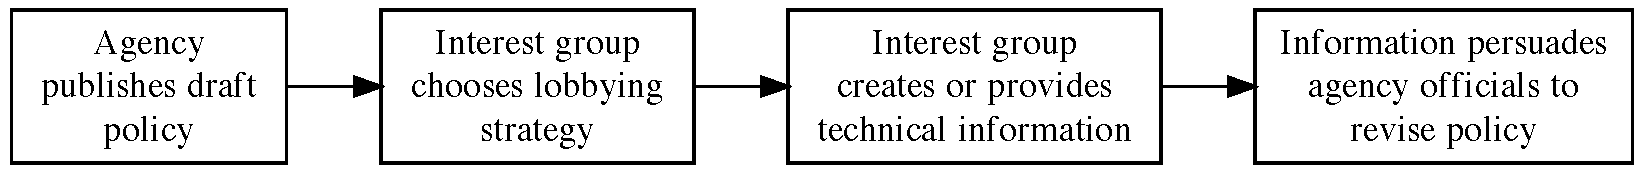
\includegraphics[width=6.5in]{../Figs/causal-classic} 

}

\caption{The 'Classic Model' of Interest Group Lobbying in Bureaucratic Policymaking}\label{fig:causal-classic}
\end{figure}

First, I offer a framework for assessing the causes of mass engagement.
Next, I argue that organizations may mobilize large numbers of people
for three reasons with observable implications for observed patterns of
mass engagement and theoretical implications for predicted effects on
policy.

\hypertarget{incorporating-political-information-into-models-of-lobbying-in-rulemaking}{%
\subsubsection{Incorporating political information into models of lobbying in rulemaking}\label{incorporating-political-information-into-models-of-lobbying-in-rulemaking}}

\hypertarget{public-pressure-campaigns-claim-to-represent-and-evoke-the-public-interest.}{%
\paragraph{Public pressure campaigns claim to represent and evoke the public interest.}\label{public-pressure-campaigns-claim-to-represent-and-evoke-the-public-interest.}}

The Oceana coalition framed its mass mobilization effort to curb the
Bureau of Ocean Energy Management's 2017 Proposed Offshore Oil and Gas
Leasing Program as a ``petition signed by 67,275 self-proclaimed United
States residents,'' suggesting that organizations consider these efforts
as akin to petitions. In the same statement, Oceana also claimed the
support of ``more than 110 East Coast municipalities, 100 Members of
Congress, 750 state and local elected officials, and 1,100 business
interests, all of whom oppose offshore drilling,'' suggesting that claims
of public and elected official support aim to provide similar kinds of
political information.

Appeals to the government are almost always couched in the language of
public interest, even when true motivations are private
\citep{Schattschneider1975}. When lobbying during rulemaking, groups often
make dubious claims to represent broad segments of the public
\citep{Seifter2016UCLA}. If agency staff do not trust an organizations'
representational claims, engaging actual people may be one of the few
credible signals of a broad base of support. Furthermore, if
organizations claim to represent people beyond their official members,
reforms requiring groups to disclose information about their funding and
membership \citep{Seifter2016UCLA} only go part way to assess groups' claims
to represent these broader segments of the public. Indeed, if advocacy
group decisions are primarily made by D.C. professionals, these
advocates themselves may be unsure how broadly their claims resonate
until potentially-attentive publics are actually engaged.

Theorists debate whether signing a petition of support without
having a role in crafting the appeal is a meaningful voice and whether
petitions effectively channel public interests, but, at a minimum,
engaging a large number of supporters may help broader interests to
distinguish themselves from truly narrower ones. It suggests that the
organization is not ``memberless'' \citep{Skocpol2003} in the sense that they
can demonstrate some verifiable public support.\footnote{Public support can be faked or inflated using ``astroturf'' tactics, but such campaigns have observably different patterns of engagement.}

\hypertarget{public-pressure-is-a-political-resource.}{%
\paragraph{Public pressure is a political resource.}\label{public-pressure-is-a-political-resource.}}

An organization's ability to expand the scope of conflict by mobilizing
a large number of people can be a valuable political resource \citep{Schattschneider1975}. In contrast to scholars who focus on the deliberative
potential of public comment processes, I focus on public engagement as a
tactic aimed at gaining power. Scholars who understand mobilization
as a tactic \citep{Furlong1997, Kerwin2011} have focused on how
organizations mobilize their membership. I expand on this understanding of mobilization as a lobbying tactic to include a campaign's broader audience, more akin to the concept of
an attentive public \citep{Key1961} or issue public \citep{Converse1964}.

Here I build on three insights. First, \citet{Furlong1997} and \citet{Kerwin2011}
identify mobilization as a tactic. The organizations that they surveyed
reported that forming coalitions and mobilizing large numbers of people
are among the most effective lobbying tactics. Second, \citet{Nelson2012}
identify political information as a potentially influential result of
lobbying by different business coalitions. While they focus on
mobilizing experts, \citet{Nelson2012} describe a dynamic that can be extended
to mass commenting:

\begin{quote}
``strategic recruitment, we theorize, mobilizes new actors to
participate in the policymaking process, bringing with them novel
technical and political information. In other words, when an expanded
strategy is employed, leaders activate individuals and organizations
to participate in the policymaking process who, without the
coordinating efforts of the leaders, would otherwise not lobby. This
activation is important because it implies that coalition lobbying can
generate new information and new actors---beyond simply the `usual
suspects'---relevant to policy decisionmakers. Thus, we theorize
consensus, coalition size, and composition matter to policy change.''
\end{quote}

I argue that, concerning political information, this logic extends to
non-experts. The number and distribution of ordinary supporters may
matter because it suggests a \emph{public} consensus. Instead of bolstering
\emph{scientific} claims, a perceived public consensus bolsters \emph{political}
claims. Finally, \citet{Furlong1998}, \citet{Yackee2006JPART}, and others distinguish
between direct and indirect forms of interest group influence in
rulemaking. This distinction is especially important for political
information, which may be most influential through indirect channels,
such as through elected officials. In short, to understand how groups
lobby in rulemaking, we must understand mass mobilization as a tactic
aimed at producing political information that may have direct and
indirect impacts on policymaking.

While most scholars have emphasized mass comments' lack of useful
technical information, a few have raised their role in creating
political information. \citet{Cuellar2005} calls on agencies to pay more
attention to ordinary peoples' expressions of preference and \citet{Rauch2016}
suggests that agencies reform the public comment process to include
opinion polls. I build from a similar intuition that mass comment
campaigns currently function like a poll or, more accurately, a
petition, capturing the intensity of preferences among the attentive
public---i.e., how many people are willing to take the time to
engage.\footnote{For example, a campaign by the World Wildlife Federation provided
  language explicitly claiming to have public opinion on their side.
  Their model comment stated that ``Along with 80\% of the American
  people, I strongly support ending commercial trade in elephant ivory
  in the US.'' This suggests that mass comment campaigns aim to signal
  information about public opinion.} Self-selection may not be ideal for representation, but
opt-in participation---whether voting, attending a hearing, or writing a
comment---may often be one of the few heuristics decisionmakers have
about public preferences.

Mobilizing citizens and generating new political information are key
functions of interest groups in a democracy
\citep{Mansbridge1992, Mahoney2007}. Campaigns inform agencies about the
distribution and intensity of opinions that are often too nuanced to
estimate a priori. Many questions that arise in rulemaking lack
analogous public opinion polling questions, making mass commenting a
unique source of political information. As with public opinion on many
specific policy issues, most members of the public and their elected
representatives may only learn about the issue and take a position as a
result of a public pressure campaign \citep{Hutchings2003}. I thus consider
public demands to be a latent factor in my model of policymaking (Figure
\ref{fig:causal-whymail}. Public demands shape the decisions of
groups who lobby in rulemaking. If they believe the attentive public is
on their side, groups may attempt to reveal this political information
to policymakers by launching a mass mobilization campaign. The public
response to the campaign depends on the extent that the attentive public
is passionate about the issue.

\begin{figure}

{\centering 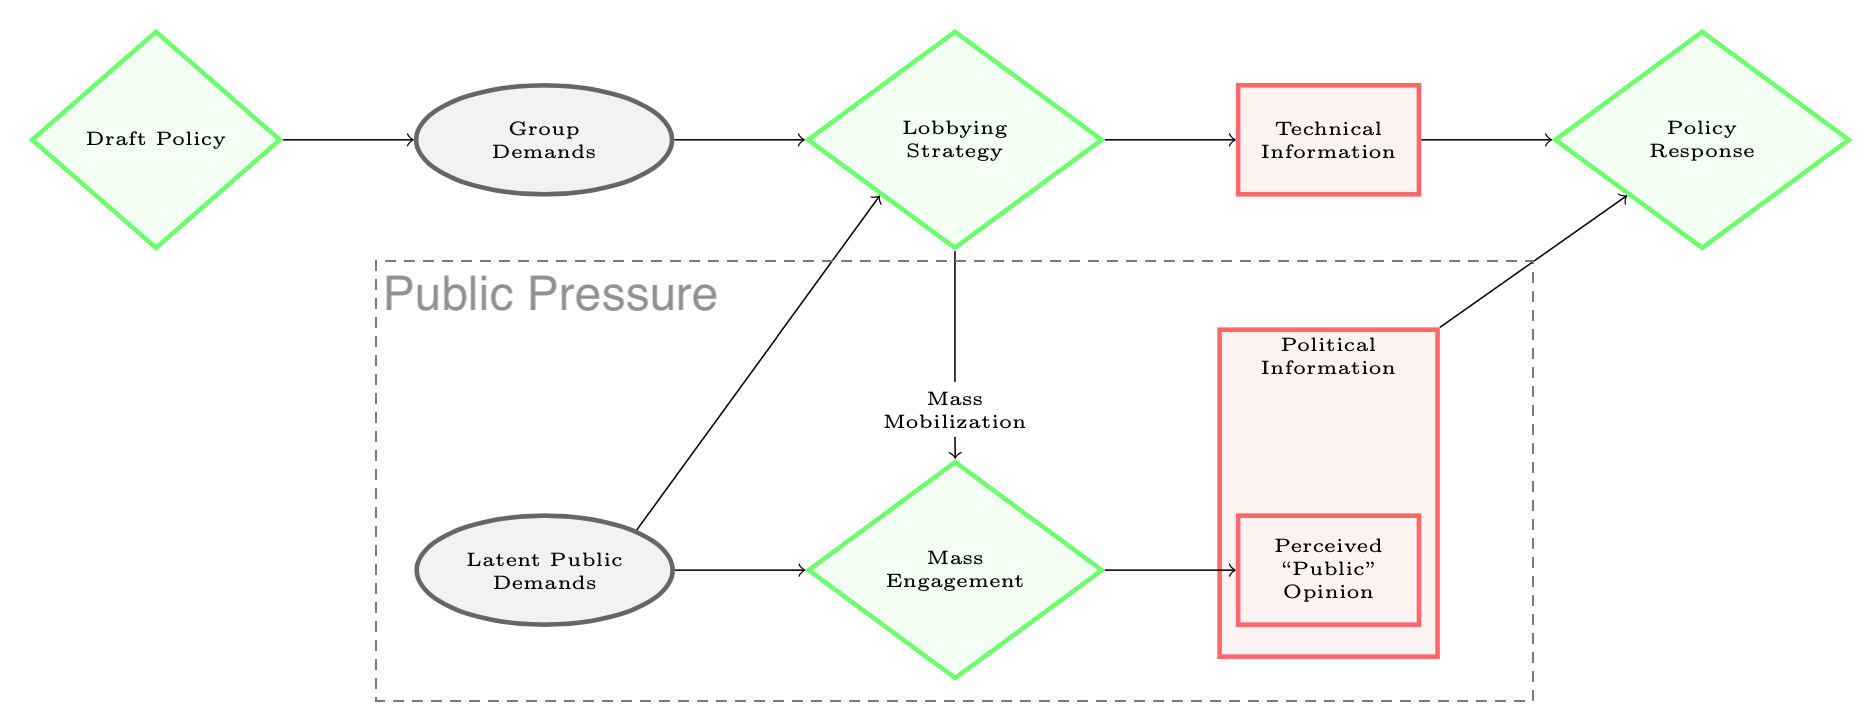
\includegraphics[width=6.5in]{../Figs/causal-whymail} 

}

\caption{Incorporating Political Information into Models of Bureaucratic Policymaking}\label{fig:causal-whymail}
\end{figure}

Figure \ref{fig:causal-whymail} amends the ``Classic Model'' of interest
group lobbying (Figure \ref{fig:causal-classic}) to incorporate political information about the attentive public. In addition to providing technical information through sophisticated comments, an organization may mobilize supporters.
The more support a group has, the more successful this mobilization effort will be.
Large-scale engagement may produce several types of relevant political
information. The most direct and obvious is the expressed ``public
opinion'' that policymakers observe.\footnote{I address other types of political information that mass engagement may create elsewhere. For an expanded model, see Figure
  \ref{fig:causal-full} in the Appendix.}

The causal process visualized in Figure
\ref{fig:causal-whymail} may only operate under certain conditions. The success of a mobilizing effort depends on whether a group's perception of latent public demands (the diagonal arrow between ``Latent Public Demands'' and ``Lobbying Strategy'') reflects the public response to a mobilizing effort (the horizontal arrow between ``Latent Public Demands'' and ``Mass Engagement'').

The influence of political information on policy (the arrow between ``Political Information'' and ``Policy Response'') depends on the institutional processes by which agencies receive and interpret information. We may only expect to observe mass mobilization influencing a particular policy only if the mobilization effort was aimed at influencing that policy, rather than using the public comment the period to build organizational membership or power more generally (see \citet{Carpenter2014b}).

\hypertarget{hypotheses-about-the-drivers-of-mass-mobilization}{%
\subsection{Hypotheses About the Drivers of Mass Mobilization}\label{hypotheses-about-the-drivers-of-mass-mobilization}}

\hypertarget{types-of-campaigns}{%
\subsubsection{Types of campaigns}\label{types-of-campaigns}}

The outcomes of mass mobilization depend, in part, on the aims of a
campaign. I distinguish group campaigns by which of three distinct aims
they pursue: (1) to win concessions by going public, (2) to disrupt a
perceived consensus, or (3) to go down fighting. Going public and
disrupting a perceived consensus are forms of proactive and reactive
outside lobbying, respectively. Here, going down fighting describes any
situation where the organization does not expect to influence policy but
mobilizes for other reasons.

\textbf{Going public.} Coalitions ``go public'' when they believe that
expanding the scope of conflict gives them an advantage.\footnote{``Going public,'' ``outside lobbying'' or an ``outside strategy''
  contrasts with insider lobbying. It is used by Presidents
  \citep{Kernell2007}, Members of Congress \citep{Malecha2012}, interest groups
  \citep{Walker1991, Dur2013}, Lawyers, and Judges (Davis 2011). For
  example, organizations may use phone banks, targeting strategies,
  and direct-mail techniques to drum-up and channel public support
  (Cooper 1985).} As these
are the coalitions that believe they have more intense public
support, mass engagement is likely to skew heavily toward this side.\footnote{This strategy is likely to be used by those disadvantaged (those
  \citet{Schattschneider1975} calls the `losers') in a policy process with
  less public attention.}
Indeed, \citet{Potter2017} finds that advocacy group-driven campaigns mobilize
far more people on average than industry-driven campaigns. Additionally,
many people may be inspired indirectly (e.g., through news stories) or
to engage with more effort (e.g., writing longer comments) than people
mobilized by the side with less public support. This is important
because political information may be especially influential if
decisionmakers perceive a consensus.\footnote{For example, the level of consensus among interest groups
  \citep{Golden1998, Yackee2006JPART}, especially business unity
  \citep{Yackee2006JOP, Haeder2015}, predicts policy change, though it is
  not clear if this is a result of strategic calculation, a perceived
  obligation due to the normative power of consensus (e.g., following
  a majoritarian logic \citep{Mendelson2011}), or simply that unified
  demands are easier to process than opposing demands.}



\begin{quote}
\textbf{Hypothesis 1a:} Lobbying coalitions
mobilize mass engagement when they perceive the attentive public is on
their side, have sufficient resources, and perceive an opportunity to
influence policy.
\end{quote}

The key part of this hypothesis is that mobilizing is correlated with
existing public support, what might be called ``grass-roots'' support. The
converse, that organizations mobilize when they have less public
support, could also be true. For example, business groups who are
already advantaged in low salience rulemaking may decide to leverage
their superior resources further to mobilize support to alter a bad
reputation or bolster claims that they represent more than their private
interest. If mobilization most often takes this ``astroturf'' form, this
would be evidence against
Hypothesis 1a and Schattschneider's argument that it is the
disadvantaged who seek to expand the scope of the conflict.

The latter parts of Hypothesis 1a regarding sufficient resources and political
opportunity are scope conditions. Most organizations that are
disadvantaged in low-salience rulemaking also lack resources to launch
mass mobilization campaigns. If an organization does not perceive a
lobbying opportunity, it would be incorrect to call mobilization a
lobbying strategy. Many factors may contribute to perceived political
opportunities. For example, \citet{Moore2017} finds that agencies that use high
levels of expertise (as defined by \citet{Selin2015}) receive fewer comments,
possibly because mobilizing organizations perceive these rules to be
less open to influence.

\textbf{Disrupting a perceived consensus.} I theorize that when coalitions
with less public support mobilize, it is a reaction to their opponents.
Because the impression of consensus is powerful, when a coalition goes
public, an opposing coalition may countermobilize. Because I theorize
that these are coalitions with less intense public support and its aim
is prevent a perceived consensus, I expect such campaigns to engage
fewer people, less effort per person, and yield a smaller portion of
indirect engagement.



\begin{quote}
\textbf{Hypothesis 1b:} When a lobbying
coalition with more intense public support mobilizes successfully in
response to an opportunity to influence policy, opposing coalitions with
less public support are more likely to countermobilize, but with
proportionally smaller results.
\end{quote}

The first part of Hypothesis 1b would be undermined if lobbying organizations
with less public support are no more likely to engage in outside
lobbying when their opponents do so. While \citet{Potter2017} found industry
groups were no more likely to advocate for rules to be strengthened,
weakened or withdrawn, this does not mean that they are no more likely
to mobilize when their opponents do so.

The second part of this hypothesis, that countermobilization is
proportionally smaller, rests on the intuition that the scale and
intensity of public engagement are moderated by preexisting support for
the proposition that people are being asked to support. It is possible
that the ``potentially mobilized'' segments of the public are unrelated to
public support before being contacted by the campaign, for example, if
mobilization is driven more by partisan identities than issue
preferences.

\textbf{Going down fighting.} Finally, campaigns may target supporters rather
than policymakers. Sometimes organizations ``go down fighting'' to fulfill
supporters' expectations. For example, \citet{Carpenter2020} finds that anti-slavery petitions were this type of campaign where ``the most important readers of a
petition are its signatories.'' In the context of notice and comment rulemaking, after a draft policy is published, failing to secure one's demands is always a loss, so I use ``going down fighting'' as shorthand for
campaigns aimed primarily at fulfilling member, donor, or supporter
expectations and related logics that are internal to the organization,
including member retention or recruitment (\citet{Carpenter2014b}, \citet{Carpenter2020}), fundraising, or satisfying a
board of directors. For example, as Figure
\ref{fig:sierra} shows, the Sierra Club uses campaigns to collect
contact information of supporters and potential members. In this case,
given the executive-branch transition between 2010 when the rule was
initiated and 2017 when it was delayed, the Sierra Club may have had
little hope of protecting methane pollution standards, but for members
of the public who wanted to voice their opinion, the Sierra Club created
an easy way to do so, as long as users consented to ``receive periodic
communication from the Sierra Club.''

\begin{figure}

{\centering 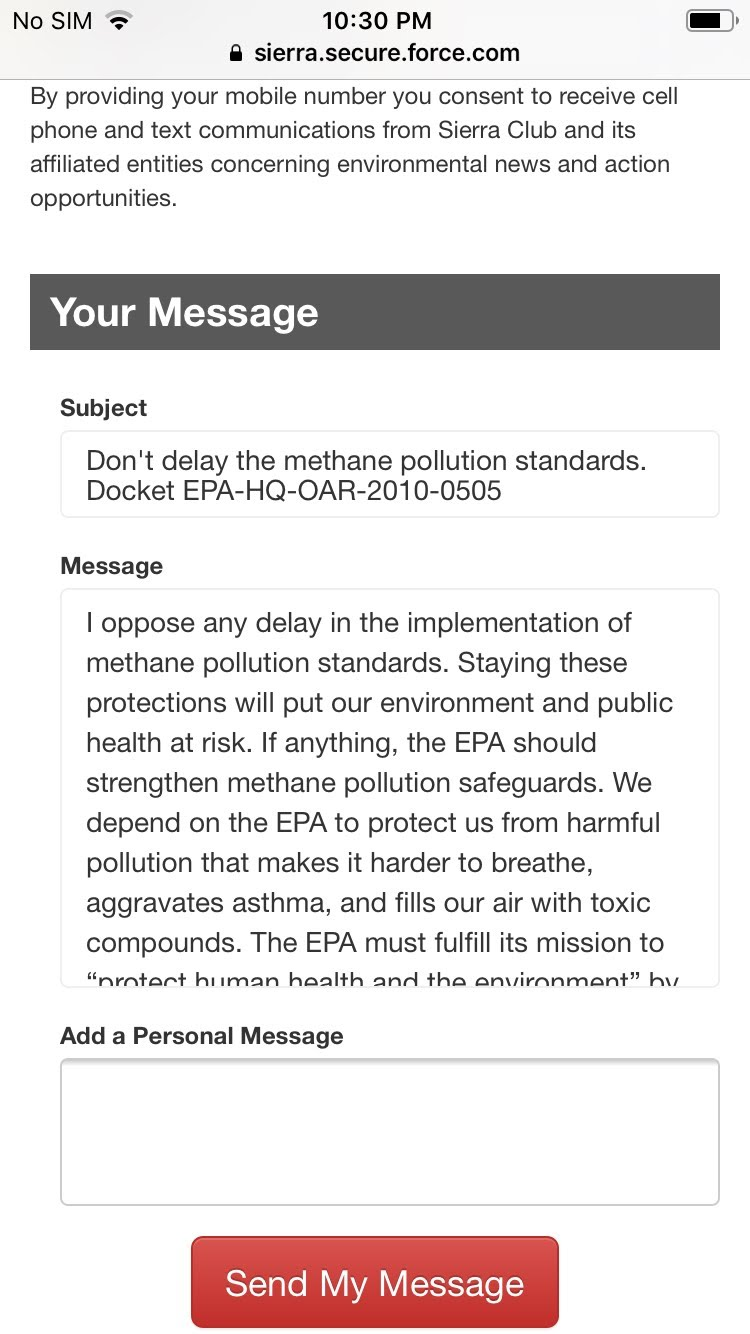
\includegraphics[width=0.4\linewidth]{/Users/devin/dissertation/Figs/sierra2} 

}

\caption{The Sierra Club Collects Contact Information Through Mass Mobilization Campaign}\label{fig:sierra}
\end{figure}

While such campaigns may engage many people, they are unlikely to affect
policy or to inspire countermobilization. I expect such campaigns to
occur on rules that have high partisan salience (e.g., rules following
major legislation passed on a narrow vote), rules that propose large
shifts on policy issues dear to member-funded public interest groups, or
rulemaking started shortly after presidential transitions when
executive-branch agendas shift more quickly than public opinion.

When a lobbying coalition with more intense public support successfully
mobilizes for reasons other than influencing policy, opposing coalitions
with less public support are not more likely to countermobilize.

Going public and going down fighting may be difficult to distinguish in
the observed public response. Indeed, members of the public may poorly
understand the different chances of success in each case. However,
lobbying organization do likely know their chances of success and should
thus invest less in sophisticated insider lobbying under the going down
fighting strategy. By identify cases where coalitions engage in large
public campaigns without corresponding investment in sophisticated
lobbying, I can assess whether countermobilization and is indeed less
likely in these cases. Table
\ref{tab:campaigns-patterns} specifies the general pattern of
engagement suggested by each of the three reasons behind mass-comment
campaigns.

\begin{longtable}[]{@{}lccc@{}}
\caption{\label{tab:campaigns-patterns} Observable Differences in Lobbying Strategies}\tabularnewline
\toprule
\begin{minipage}[b]{0.19\columnwidth}\raggedright
\strut
\end{minipage} & \begin{minipage}[b]{0.23\columnwidth}\centering
Inside lobbying (eg., technical information provided)\strut
\end{minipage} & \begin{minipage}[b]{0.23\columnwidth}\centering
Outside lobbying (e.g., the number of comments from a public pressure campaign)\strut
\end{minipage} & \begin{minipage}[b]{0.23\columnwidth}\centering
\strut
\end{minipage}\tabularnewline
\midrule
\endfirsthead
\toprule
\begin{minipage}[b]{0.19\columnwidth}\raggedright
\strut
\end{minipage} & \begin{minipage}[b]{0.23\columnwidth}\centering
Inside lobbying (eg., technical information provided)\strut
\end{minipage} & \begin{minipage}[b]{0.23\columnwidth}\centering
Outside lobbying (e.g., the number of comments from a public pressure campaign)\strut
\end{minipage} & \begin{minipage}[b]{0.23\columnwidth}\centering
\strut
\end{minipage}\tabularnewline
\midrule
\endhead
\begin{minipage}[t]{0.19\columnwidth}\raggedright
``Normal'' lobbying\strut
\end{minipage} & \begin{minipage}[t]{0.23\columnwidth}\centering
High\strut
\end{minipage} & \begin{minipage}[t]{0.23\columnwidth}\centering
None\strut
\end{minipage} & \begin{minipage}[t]{0.23\columnwidth}\centering
\strut
\end{minipage}\tabularnewline
\begin{minipage}[t]{0.19\columnwidth}\raggedright
``Going public''\strut
\end{minipage} & \begin{minipage}[t]{0.23\columnwidth}\centering
High\strut
\end{minipage} & \begin{minipage}[t]{0.23\columnwidth}\centering
High\strut
\end{minipage} & \begin{minipage}[t]{0.23\columnwidth}\centering
\strut
\end{minipage}\tabularnewline
\begin{minipage}[t]{0.19\columnwidth}\raggedright
``Disrupting consensus''\strut
\end{minipage} & \begin{minipage}[t]{0.23\columnwidth}\centering
High\strut
\end{minipage} & \begin{minipage}[t]{0.23\columnwidth}\centering
Low\strut
\end{minipage} & \begin{minipage}[t]{0.23\columnwidth}\centering
\strut
\end{minipage}\tabularnewline
\begin{minipage}[t]{0.19\columnwidth}\raggedright
``Going down fighting''\strut
\end{minipage} & \begin{minipage}[t]{0.23\columnwidth}\centering
Low\strut
\end{minipage} & \begin{minipage}[t]{0.23\columnwidth}\centering
High\strut
\end{minipage} & \begin{minipage}[t]{0.23\columnwidth}\centering
\strut
\end{minipage}\tabularnewline
\bottomrule
\end{longtable}

As Table
\ref{tab:campaigns-patterns} suggests, the relevant statistic
distinguishing patterns is the \emph{relative} number of each type of comment
on each side on a given rulemaking docket. Even among rules targeted by
campaigns, salience varies significantly and thus ``high'' and ``low''
numbers of comments will differ across rules. Importantly, even
campaigns that achieve very low public response rates appear in these
data. Because campaigns aim to collect thousands of comments, it is
implausible that even the most unpopular position would achieve no
supportive responses. For example, \citet{Potter2017} found Poultry Producers
averaging only 319 comments per campaign. While this is far from the
Sierra Club's average of 17,325 comments per campaign, it is also far
from zero.

\hypertarget{public-and-private-goods.}{%
\paragraph{Public and private goods.}\label{public-and-private-goods.}}

While coalitions may form around various material and ideological
conflicts, those most likely to be advantaged by going public or going
down fighting are public interest groups---organizations primarily
serving an idea of the public good rather than the material interests of
their members.\footnote{\citet{Potter2017} similarly distinguishes ``advocacy groups'' from
  ``industry groups.'' \citet{Berry1999} calls these groups ``citizen groups''
  and emphasizes conflict over cultural issues. While some public
  interest groups focus on conservative or progressive cultural
  issues, like religious education, immigration, or endangered
  species, many are more focused on the public provision or protection
  of public goods such as national parks, consumer product safety
  standards, air quality, drinking water, and public safety.
  One exception may be types of membership organizations that are both
  broad and often focused on material outcomes for their members such
  as labor unions. \citet{Potter2017} puts unions in the ``Industry'' category.
  I take a different approach based on the coalition with whom such
  groups lobby. If a union lobbies alongside businesses (see \citet{Mildenberger2020}), I classify
  this as a private interest-driven coalition. If a union lobbies with
  public interest groups on public health or safety issues, I classify
  this as a public interest.} Thus, I theorize that mass mobilization is most
likely to occur in conflicts of public versus private interests or
public versus public interests (i.e., between coalitions led by groups
with distinct cultural ideals or desired public goods), provided they
have sufficient resources to run a campaign. If true, one implication is
that mass mobilization will systematically run counter to concentrated
business interests where they conflict with the values of public
interest groups with sufficient resources to mobilize.



\begin{quote}
\textbf{Hypothesis 1c:} Public interest group coalitions mobilize more often than
business-driven coalitions.
\end{quote}

Hypothesis 1c posits a conditional logic in the
decision to mobilize. If resources purely determined outside lobbying,
business-driven coalitions would often dominate, as they do elsewhere.
However, I argue, because outside lobbying can alter the decision
environment, those who have the advantage in the usual rulemaking
process (where a more limited set of actors participate) have little
incentive to expand the scope of the conflict.

\hypertarget{types-of-public-engagement}{%
\subsection{Types of public engagement}\label{types-of-public-engagement}}

I classify supporters into three types that help describe key pieces of
political information. I illustrate these types in the context of public
comments. Comments that are exact copies of a form letter are akin to
petition signatures from supporters who were engaged by a campaign to
comment with minimal effort. Commenters that also take time to add text
indicate more intense preferences. Finally, commenters who express
solidarity in similar but distinct phrases indicate they were engaged
indirectly, perhaps by a news story or a social media post about the
campaign, as campaign messages spread beyond those initially
targeted.\footnote{It is possible that some people in this latter category engage
  purely on their own initiative, but any impact they have likely
  comes from their alignment with a coalition. Furthermore, as I show
  below, wholly original comments are rare.} Because the success of a mobilization effort is moderated
by public support, broader public interest group coalitions ought to
mobilize more people, more effort per person, and more people indirectly
for the same amount of mobilization effort (e.g., spending or
solicitations).

Public interest group coalitions mobilize more successfully than
business-driven coalitions. Indicators of success include (1) the number
of comments supporting a coalition (2) the effort per comment (3) the
number of comments mobilized indirectly.

The size of each group thus offers political information to
policymakers, including coalition resources, the intensity of sentiment,
and the potential for conflict to spread. The first two types signal two
kinds of intensity or resolve. First, they show the mobilizers'
willingness to commit resources to the issue. Second, costly actions
show the intensity of opinions among the mobilized segment of the public
\citep{Dunleavy1991}. The number of people engaged by a campaign is not
strictly proportional to an organization's investment. The less people
care, the more it costs to mobilize them. The third type indicates
potential contagion. Indications that messages spread beyond those
initially targeted may be especially powerful \citep{Kollman1998}.

Information about organizational resolve, the intensity of public
demands, and contagiousness are thus produced, but such political
information will only influence decisions if these signals are processed
in a way that captures this information and relays it to decisionmakers.
These organizational processes may vary significantly across agencies.

\hypertarget{whyMail-methods}{%
\section{Methods}\label{whyMail-methods}}

\hypertarget{measuring-public-pressure-and-political-information}{%
\subsection{Measuring Public Pressure and Political Information}\label{measuring-public-pressure-and-political-information}}

In this section, I develop methods to attribute mass comments to the
campaigns that mobilized them and measure the intensity of preferences
expressed. To link individual comments to the more sophisticated
lobbying efforts they support, I use textual similarity to identify
clusters of similar comments, reflecting formal and informal coalitions.
Comments with identical text (if any) indicate which groups and
coalitions ran a mass comment campaign. Within each campaign, I measure
the intensity and potential for the movement to grow. To measure
intensity, I examine the ratio of high-effort and low-effort comments.
To measure the potential to grow, I measure the number of comments mobilized
indirectly by the campaign (i.e., those that support a campaign but do
not include text provided by the campaign). The result is several new
measures of participation in bureaucratic policymaking.

\hypertarget{data.}{%
\paragraph{Data.}\label{data.}}

I collected a corpus of approximately 70 million comments via the
regulations.gov API. About 50 million of these comments are on proposed
rules (over 16,000 proposed rules from 144 agencies from 2005 to 2018).
I then linked these comments to other data on the rules from the Unified
Agenda and Office of Information and Regulatory Affairs Reports on draft
rules sent to them for review. Summary statistics for these data are
available in the Appendix.

\hypertarget{who-lobbies}{%
\subsubsection{Who lobbies?}\label{who-lobbies}}

Unfortunately, metadata on the authors of comments and their
organizational affiliations are inconsistent and incomplete. As this
information is key to identifying influential actors, improving these
data was a significant data-organization task.

\hypertarget{mobilizing-organizations.}{%
\paragraph{Mobilizing organizations.}\label{mobilizing-organizations.}}

Through an iterative combination of automated search methods and hand-coding, I identify organizations for over 40 million comments, including all organizations responsible for mobilizing 100 or more
comments with repeated text--either identical text or partially unique
texts that contain shared language. I then searched comment texts for
mentions of these organizations' names to complete missing information
on the mobilizing organization. The top 100 mobilizing organizations
each mobilized between 55 thousand and 4.2 million comments. Figure
\ref{fig:toporgs} shows the top organizers of comments posted to
regulations.gov.

\begin{figure}

{\centering 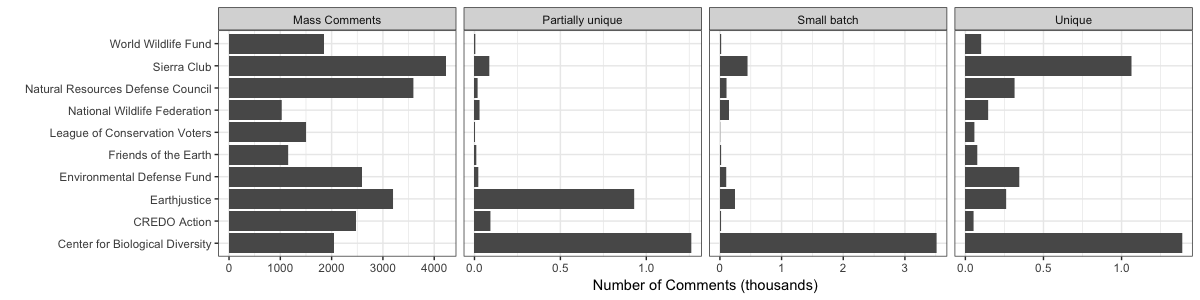
\includegraphics[width=6.5in]{../Figs/toporgs} 

}

\caption{Top mobilizers of comments posted to regulations.gov}\label{fig:toporgs}
\end{figure}

\hypertarget{who-lobbies-together}{%
\subsubsection{Who lobbies together?}\label{who-lobbies-together}}

Having identified who is participating in rulemaking, the next step is
to determine who is lobbying together. Studies of rulemaking stress the importance of coalitions \citep[Dwidar2019]{Yackee2006JOP}. Scholars have measured coalitions of organized groups but have yet to attribute citizen comments to the coalition that mobilized them.

\hypertarget{i-identify-coalitions-using-text-re-use-and-clustering-methods.}{%
\paragraph{I identify coalitions using text re-use and clustering methods.}\label{i-identify-coalitions-using-text-re-use-and-clustering-methods.}}

I identify comments that are not identical but share a 10-word (or
``10-gram'') string using a moving window function looping over each
possible pair of texts to identify matches.\footnote{For more about this method and comparisons with related partial matching methods such as the Smith-Waterman algorithm, see \citet{Casas2017} and \citet{Judge-Lord2017}.}
When actors sign onto the same comment, it is clear that they are
lobbying together. However, various businesses, advocacy groups, and
citizens often comment separately, even when they are aligned. Thus, in addition to mapping text re-use, for rules with a large number of comments,
I use statistical models of text to classify comments into coalitions. I cluster
documents by the frequency with which they use different words. Being
classified together does not mean that the documents all address exactly
the same distribution of substantive issues, just that they use similar
words relative to the full set of documents. I start by modeling all
comments on each rule (collapsing identical comments to one document)
with two and three clusters, which I then inspect to see how well the
comments of named organizations were classified. If the two cluster
model most sensibly describes the conflict, I label these clusters ``pro'' and ``con'' If the three-cluster model more sensibly describes the
conflict, I label these clusters as ``pro, con, other.'' If neither fits
well, I increase the number of clusters as needed.

\begin{figure}

{\centering 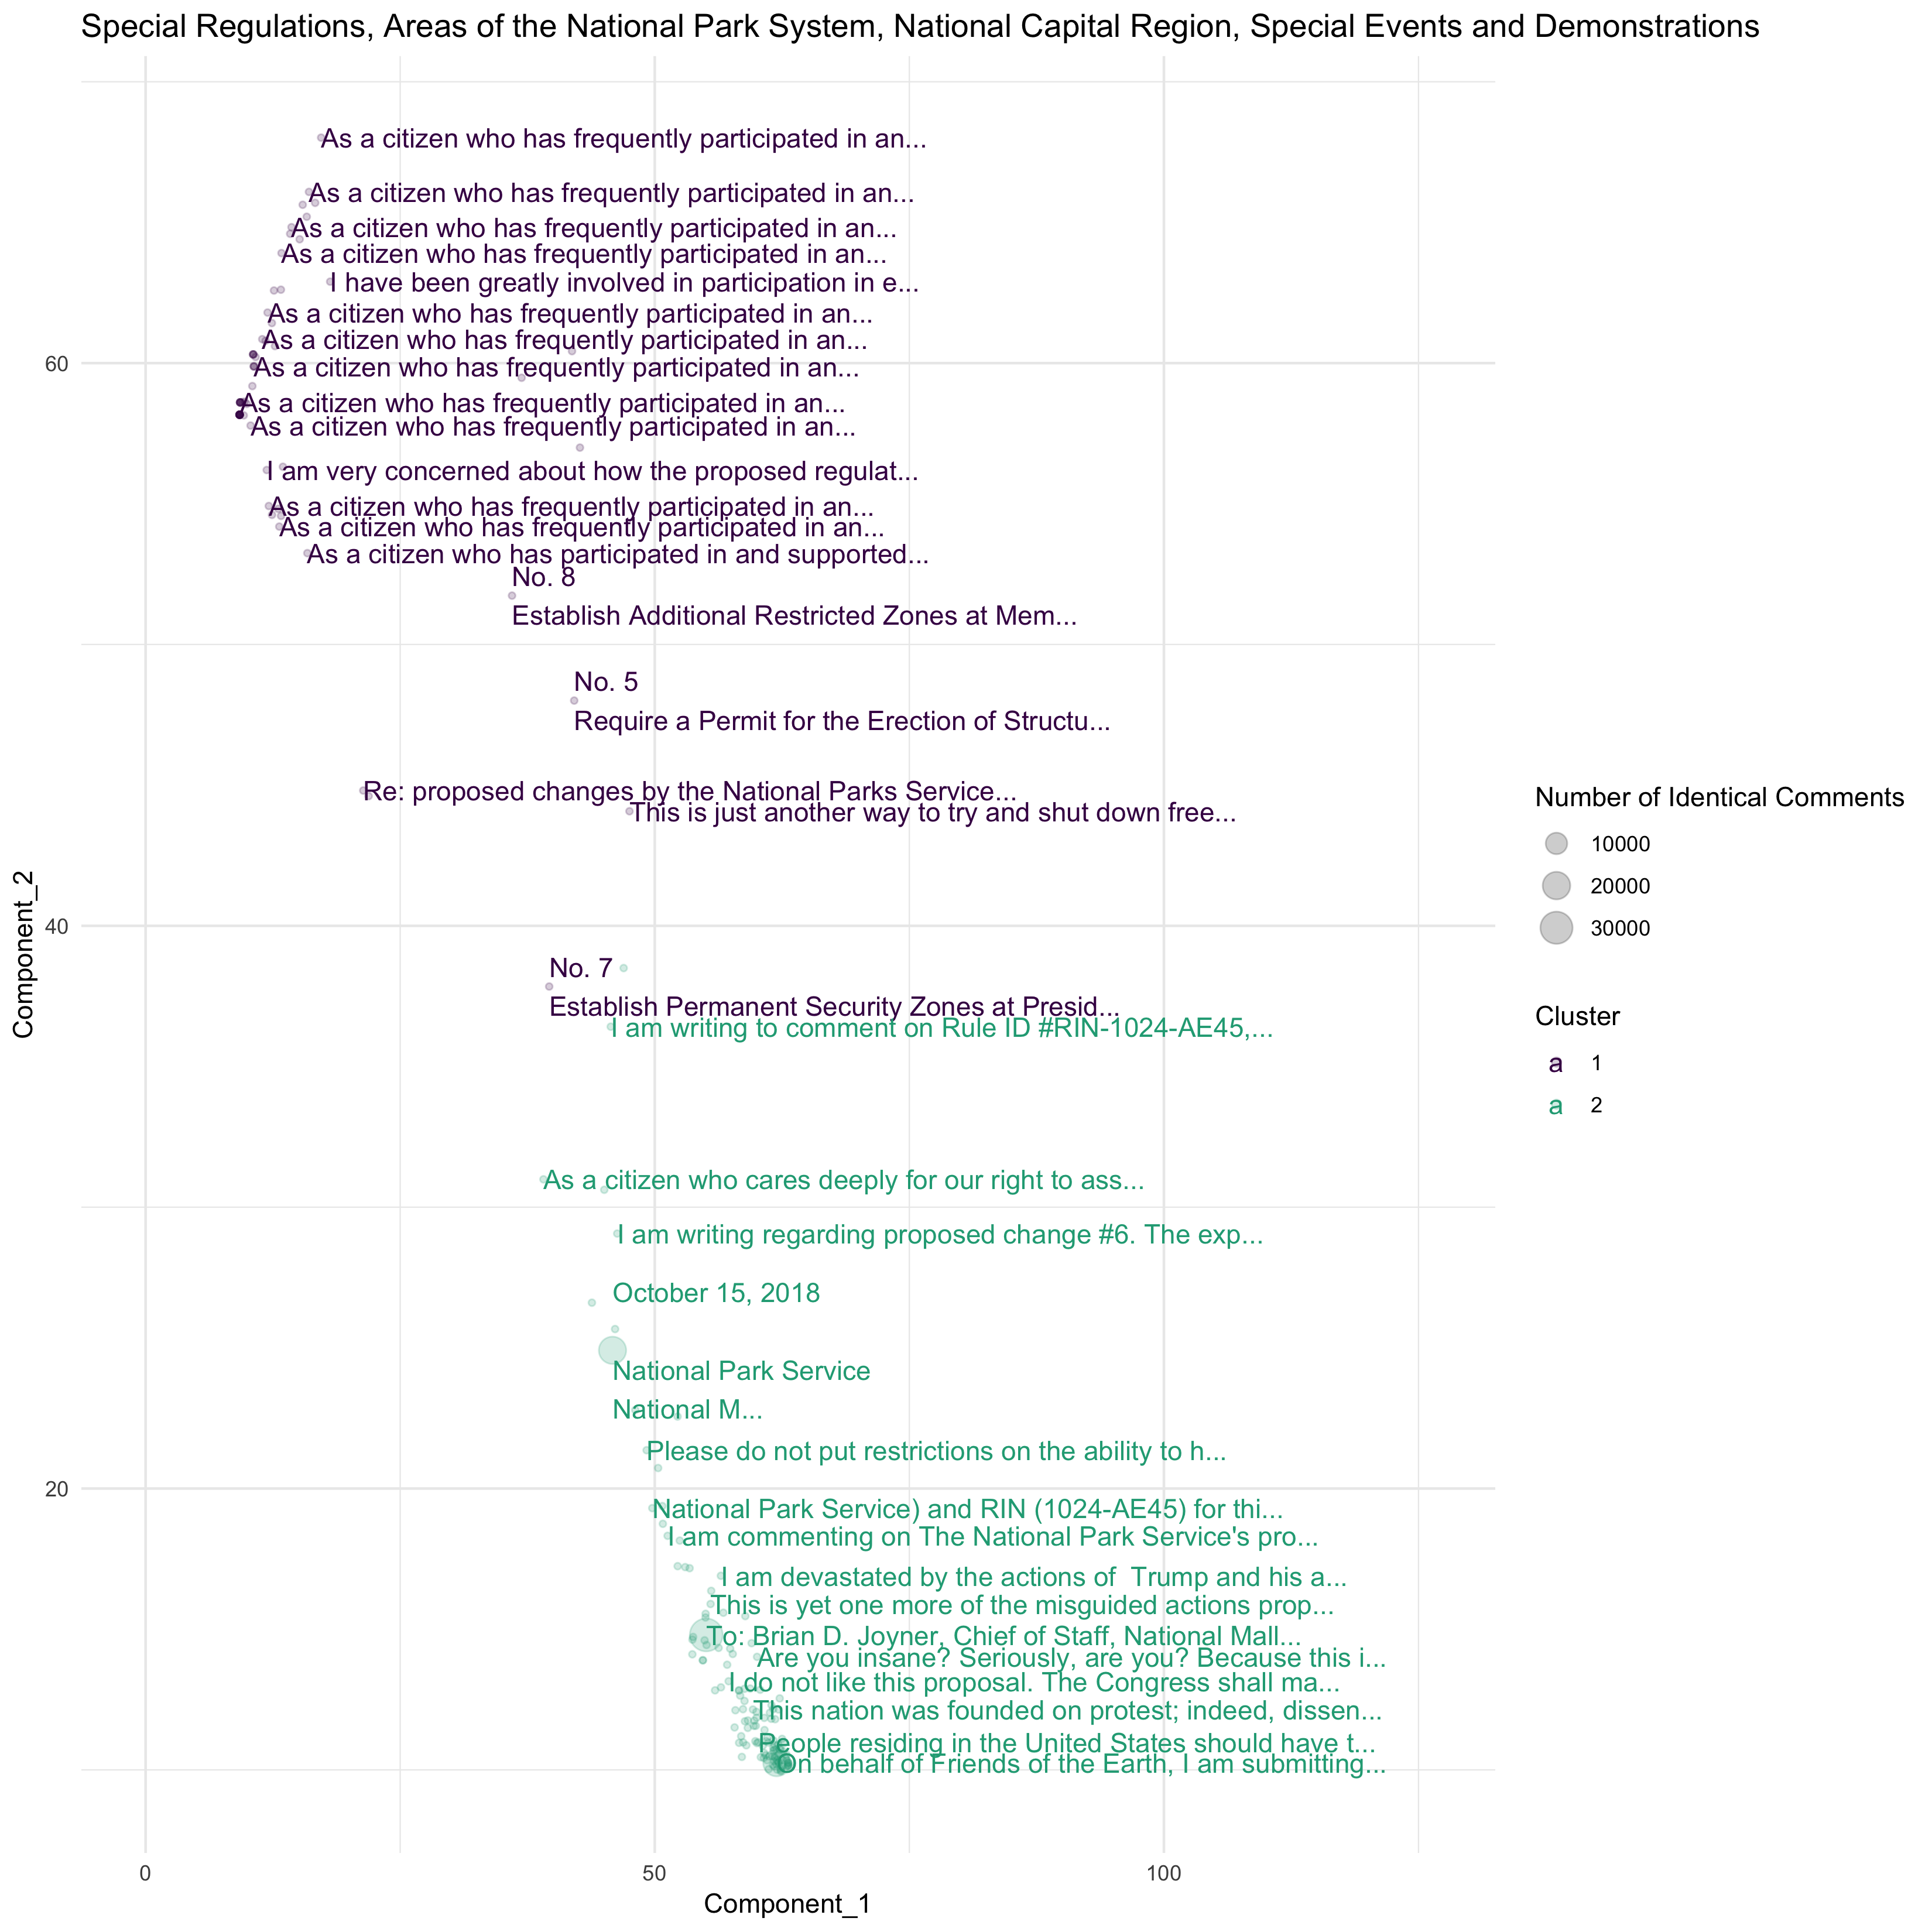
\includegraphics[width=6.5in]{../Figs/kmeans} 

}

\caption{K-means clustering fails to capture coalitions when nearly all comments oppose a regulation}\label{fig:kmeans}
\end{figure}

The asymmetry in expressed support for most rules presents challenges
for unsupervised clustering because much of the variation in comment
texts is within-coalition variation. For example, one of the most common
clustering methods, k-means clustering, often captures within-coalition
variation. Figure \ref{fig:kmeans} shows k-means clusters based on a normalized
measure of word frequency (term-frequency/inverse-document-frequency)
compared to two principal components of variation. Neither k-means nor
principal components analysis is well suited to identifying the small
number of comments supporting the Park Service's proposed restrictions
on protests in Washington DC.

Two strategies may improve clustering. First, even partial text re-use
generally indicates that comments belong to the same coalition. For
example, as seen at the top of Figure
\ref{fig:kmeans}, models
may be restricted to cluster the large number of comments beginning with
``As a citizen who has frequently participated'' in the same coalition
even if they go on to add different personal anecdotes about why protest
rights are important to them. Thus, clustering methods could be
restricted to group partially copied texts, as well as entirely copied
texts. Second, Bayesian mixture model may better recover pro and con
clusters, especially with strong priors comments using positive and
negative sentiment words belong together.

\hypertarget{measuring-the-volume-intensity-and-potential-contagion-of-public-engagement.}{%
\subsubsection{Measuring the volume, intensity, and potential contagion of public engagement.}\label{measuring-the-volume-intensity-and-potential-contagion-of-public-engagement.}}

I measure variation in engagement in three ways, corresponding to the
three types of comments described above.

\textbf{Volume.} First, I measure the total number of comments on the rule.
As commenting results from multiple processes: a coalition deciding to
lobby at all, a coalition deciding to mobilize, and response to the
campaign the distribution contains many cases where groups may have had
success mobilizing but never reached the choice of whether to mobilize
or not. Perhaps they were unaware of the draft rule. Once the decision
to mobilize has been reached and made, the response to mobilizing is a
count process. Thus, I expect the count of comments across rules to
follow a zero-inflated negative binomial distribution.

\textbf{Effort.} I measure effort per comment by the number of words people
write, omitting any to text longer than ten words that is not unique,
usually because a mobilizing organization provided it. For example, the Sierra Club mobilized more than 47,710
people to submit exactly the same text on the delay of the methane
pollution rule, but 7,452 people also took the time to write a
personalized comment in addition to the text provided (see Figure \ref{fig:sierra}). However, we may
not observe people who have low levels of passion for the issue because
they either do not cross the effort threshold required to comment or opt
to write nothing more than the form letter. Thus, while effort measured
by the number of words people write may be normally distributed, I
assume that the low end of the observed distribution is truncated.

\textbf{Contagion.} Mass-comment campaigns have wildly different results.
Some submit a clean 10,000 copies of (signatures on) the same comment.
Others ``go viral''---inspiring a mess of further engagement where the
original messages are translated through social media posts and news
stories. To identify people who were plausibly mobilized indirectly by a
campaign, I count the number of people who use a similar distribution of
words to that of the form letter but fewer than ten words matching any
other comment. This is a regular count process.

\hypertarget{whyMail-results}{%
\section{Results: Patterns of Public Engagement in Rulemaking}\label{whyMail-results}}

\hypertarget{patterns-of-public-engagement-in-rulemaking}{%
\subsection{Patterns of public engagement in rulemaking}\label{patterns-of-public-engagement-in-rulemaking}}

\hypertarget{most-comments-result-from-mass-comment-campaigns.}{%
\paragraph{Most comments result from mass-comment campaigns.}\label{most-comments-result-from-mass-comment-campaigns.}}

Figure
\ref{fig:comments-support} shows all comments posted on
regulations.gov over time by whether they are exact or partial copies of
another comment or not. I call comments that have between 2 and 99
identical copies, ``medium batch'' because such comments may reflect
coordinated efforts among interest groups that do not include a public
pressure strategy that involves mobilizing ordinary people. Even relatively unsuccessful public pressure campaigns yield far more than 99 comments. Comments that have either 100 or more identical copies or were uploaded in bulk batches of at least 100 are then ``mass comments'' that were certainly mobilized by a public pressure campaign. Figure \ref{fig:comments-support} shows that public pressure campaigns mobilize the vast majority of comments. Over 80\% of the 48 million comments on proposed rules posted to regulations.gov were mobilized by just 100 organizations. In other words, most comments are from ordinary people mobilized by a few public interest organizations.

\begin{figure}

{\centering 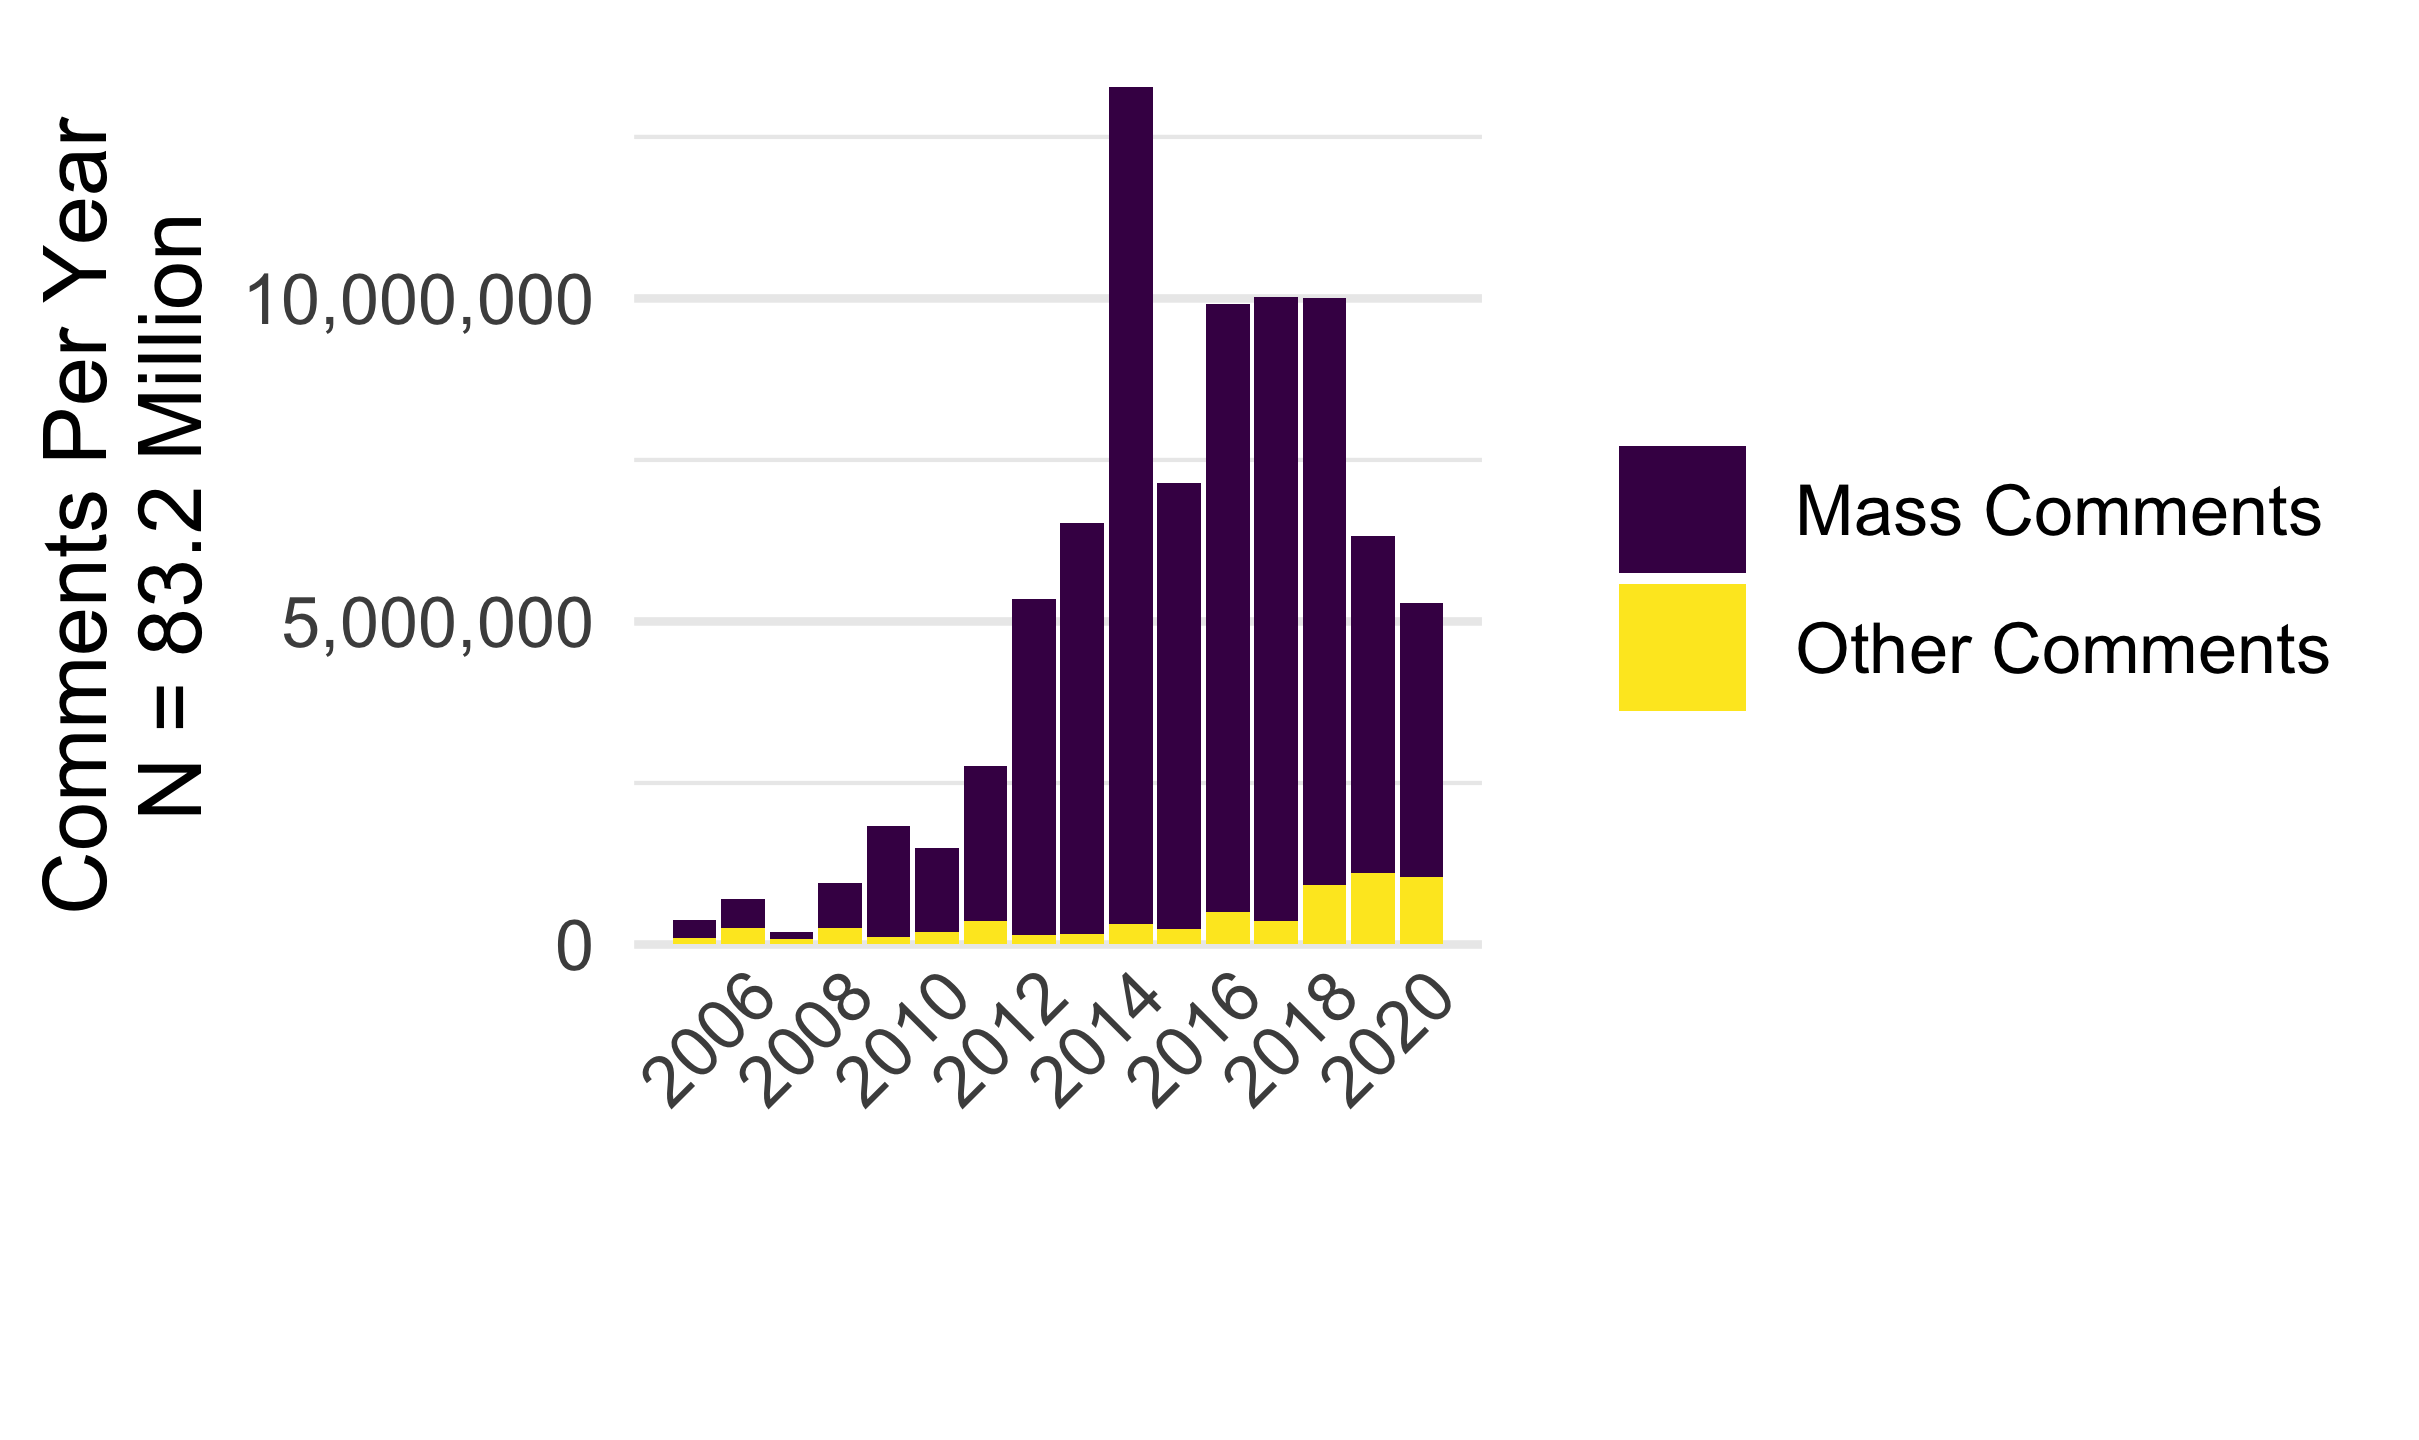
\includegraphics[width=0.49\linewidth]{../Figs/comments-mass-1} 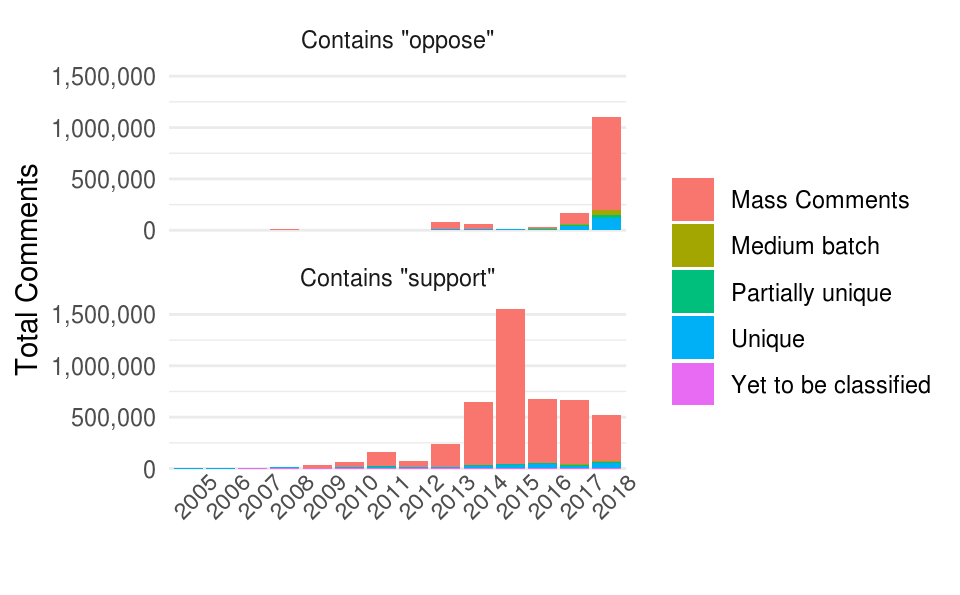
\includegraphics[width=0.49\linewidth]{../Figs/comments-mass-support-vs-oppose-1} 

}

\caption{Comments on Draft Rules Posted to Regulations.gov 2006-2018}\label{fig:comments-support}
\end{figure}

The right pane of Figure
\ref{fig:comments-support} shows results from a sample of several
million comments for which I have digitized texts. Many of these
comments appear to support proposed agency rules. A rough measure of
support (whether the comment text includes " support " or " oppose ``)
shows that many more comments mention support, until 2018 when there is
a fairly dramatic reversal in the share of comments mentioning''support
" compared to those mentioning ``oppose'' (Figure
\ref{fig:comments-support}. This may be a function of the
changing regulatory agenda due to the change in presidential
administration. However, support and oppose are not used in all comments
and do not always indicate support for a rule (see figures
\ref{fig:sentiment-2018} and
\ref{fig:sentiment-2016} in the appendix for a sample of comments
on several rules in 2016 and 2018).

\hypertarget{most-comments-occur-on-a-small-number-of-salient-rules.}{%
\paragraph{Most comments occur on a small number of salient rules.}\label{most-comments-occur-on-a-small-number-of-salient-rules.}}

Approximately one-third of public comments posted to regulations.gov
were received on just ten regulations shown in Figure
\ref{fig:topdockets}.

\begin{figure}

{\centering 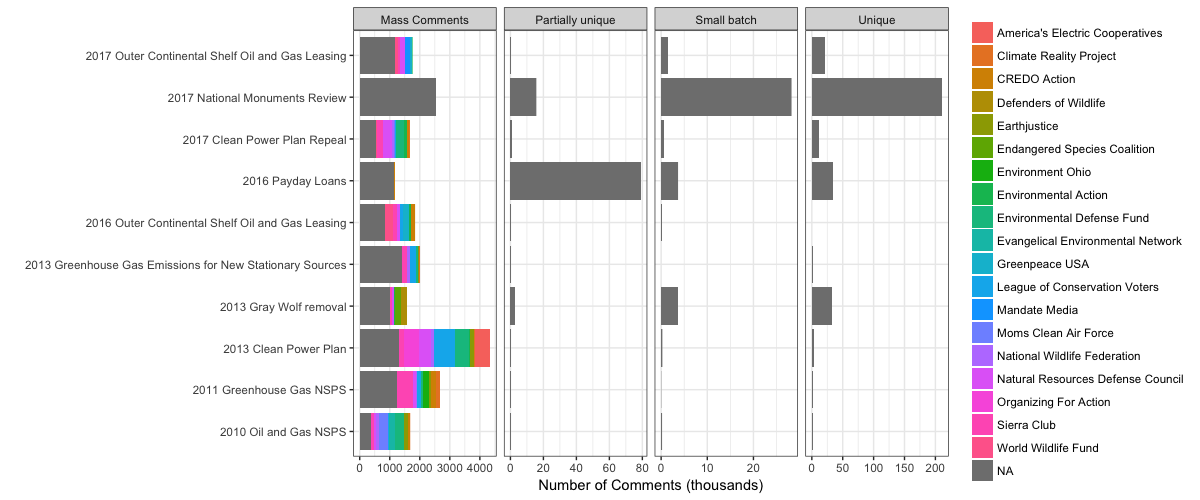
\includegraphics[width=6.5in]{../Figs/topdockets} 

}

\caption{Top 10 Dockets Receiving the Most Comments on regulations.gov and the top 20 Mobilizers}\label{fig:topdockets}
\end{figure}

\hypertarget{is-civic-engagement-resulting-from-public-pressure-campaigns-better-understood-as-astroturf-or-grassroots-participation}{%
\subsubsection{Is civic engagement resulting from public pressure campaigns better understood as ``astroturf'' or ``grassroots'' participation?}\label{is-civic-engagement-resulting-from-public-pressure-campaigns-better-understood-as-astroturf-or-grassroots-participation}}

In short, I find much more evidence of grassroots participation than astroturf participation.

\hypertarget{a-coalition-of-public-interest-organizations-mobilize-most-comments.}{%
\paragraph{A coalition of public-interest organizations mobilize most comments.}\label{a-coalition-of-public-interest-organizations-mobilize-most-comments.}}

As Figure \ref{fig:topdockets} shows, the most prolific mobilizers are
environmental groups. On five out of the top ten dockets (here including
rulemaking and non-rulemaking dockets), a similar coalition of groups
mobilized the majority of public comments. In part, this is because the
Environmental Protection Agency produces a large share of the
substantive rules posted to regulations.gov. However, it is notable
that, on the top ten dockets, 19 of the top 20 mobilizers generally
lobby together. America's Energy Cooperatives (AEC), an industry association,
stands out as the lone mobilizer on behalf of material interest for its
members. Notably, it only mobilized significantly on the Clean Power
Plan but not on the subsequent Clean Power Plan repeal. If public
interest group mobilizing on the Clean Power Plan was an example of
``going public'' to pressure the Obama administration and then ``going
down fighting'' in the face of the Trump administration's repeal,
industry counter-mobilization responding to the first, but not the
second aligns with Hypothesis 1b. If AEC found their policy goals in the Clean Power Plan rulemaking threatened by the political information being generated by environmental groups, it would make sense to devote resources to their own public pressure campaign to disrupt any perceived consensus. Likewise, if AEC was not concerned that environmental group mobilizing would affect the Clean Power Plan repeal, sponsoring a public pressure campaign would be a poor investment.

\hypertarget{conclusion}{%
\section{Conclusion}\label{conclusion}}

The legitimacy of bureaucratic policymaking is said to depend on the premise that rulemaking provides for public voice \citep[\citet{Rosenbloom2003}]{Croley2003}. Yet we lack an empirical base necessary to evaluate whether any legitimacy the public comment process may provide is deserved. If input solicited from ordinary people has little effect on policy outcomes, directly or indirectly, it may be best understood as providing a veneer of democratic legitimacy on an essentially technocratic and/or elite-driven process. I have made a few initial steps toward better understanding actual public engagement in bureaucratic policymaking.
If public pressure campaigns do shape agency decisions, a new research program will be needed to investigate who exactly these campaigns mobilize and represent.

\newpage

\hypertarget{appendix-appendix}{%
\appendix}


\hypertarget{appendix}{%
\section*{Appendix}\label{appendix}}
\addcontentsline{toc}{section}{Appendix}

\begin{figure}

{\centering 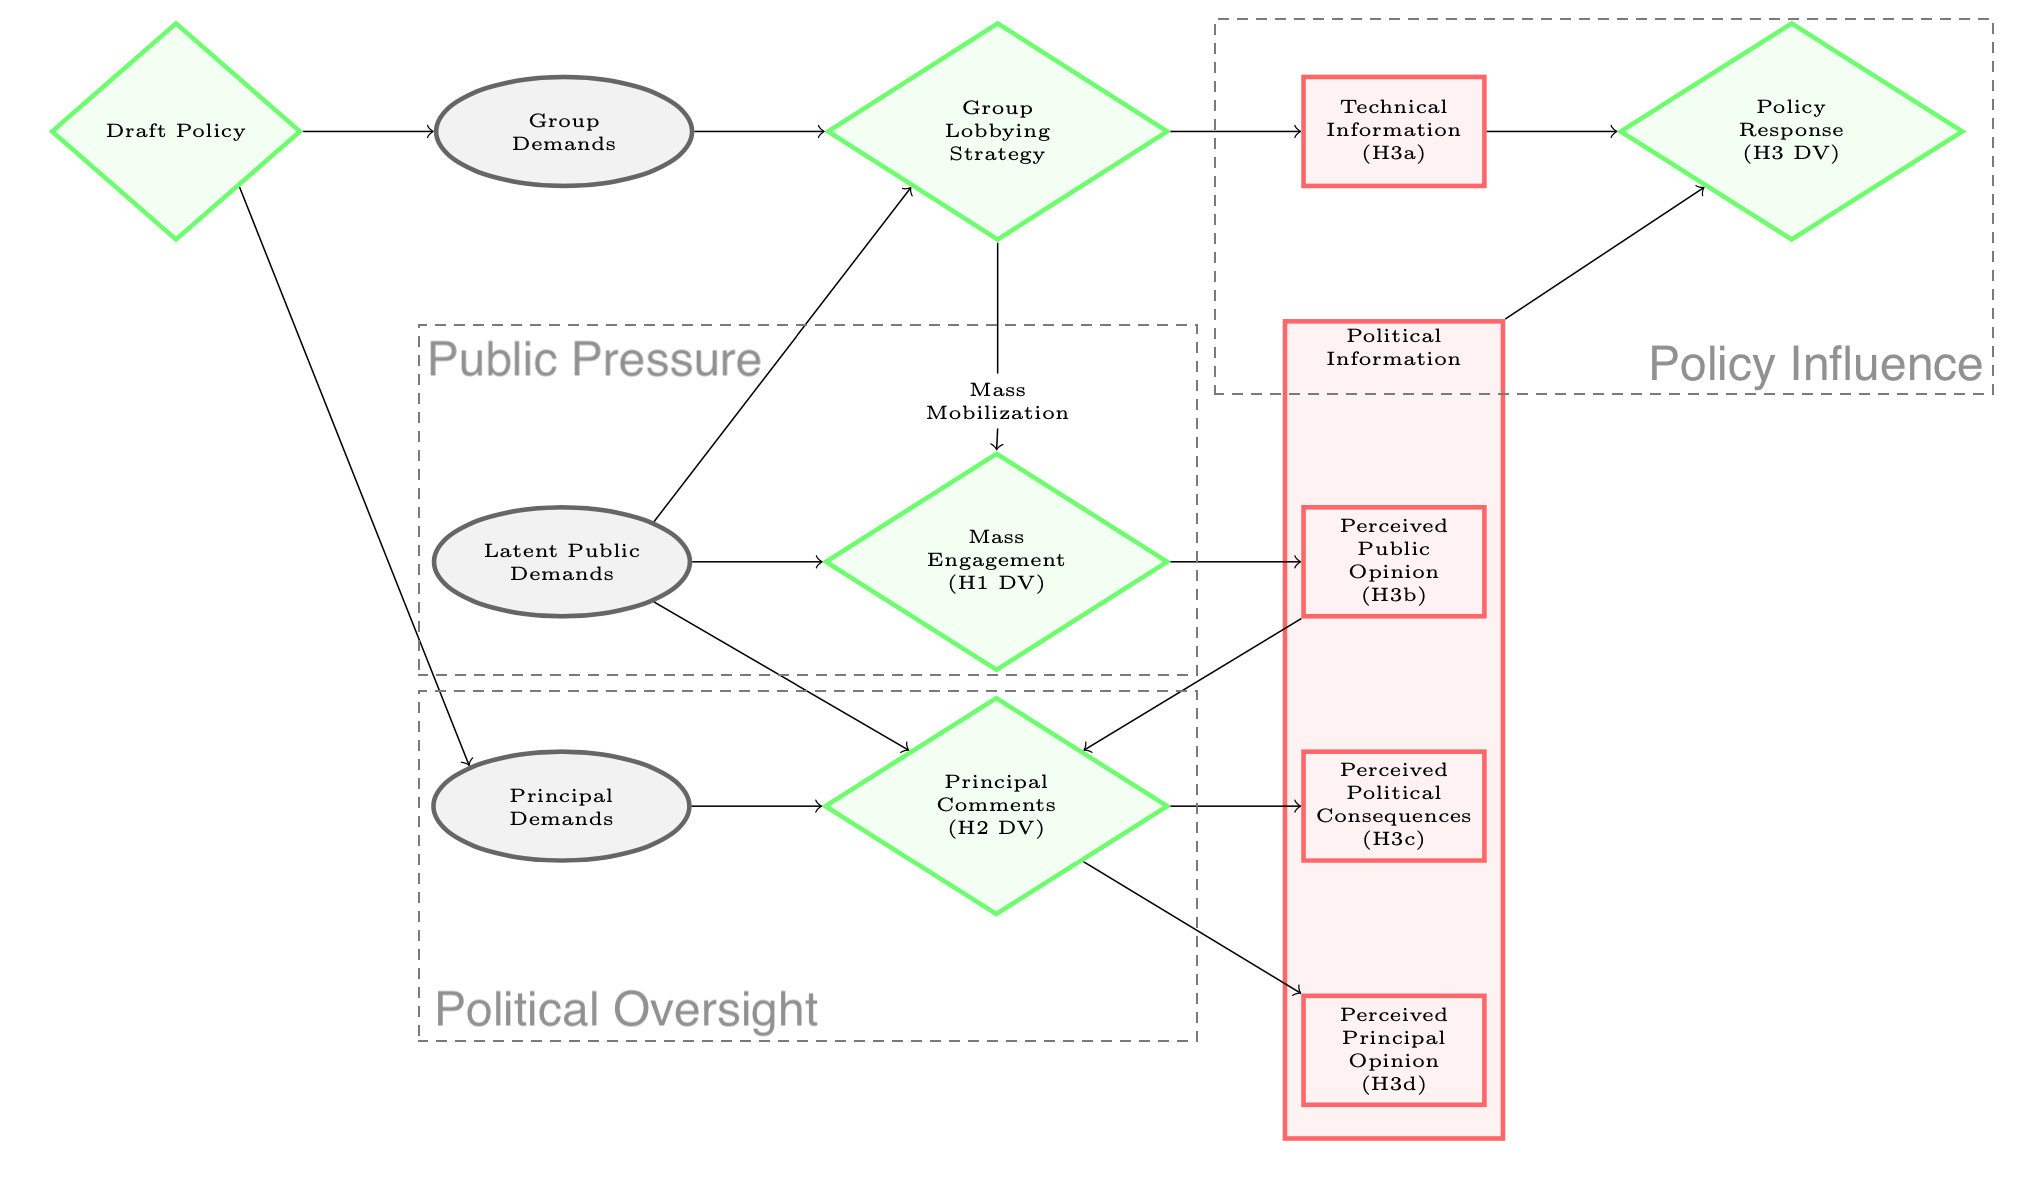
\includegraphics[width=6.5in]{../Figs/causal-full} 

}

\caption{The Role of Mass Commenting and Political Information in Bureaucratic Policymaking}\label{fig:causal-full}
\end{figure}

\begin{figure}

{\centering 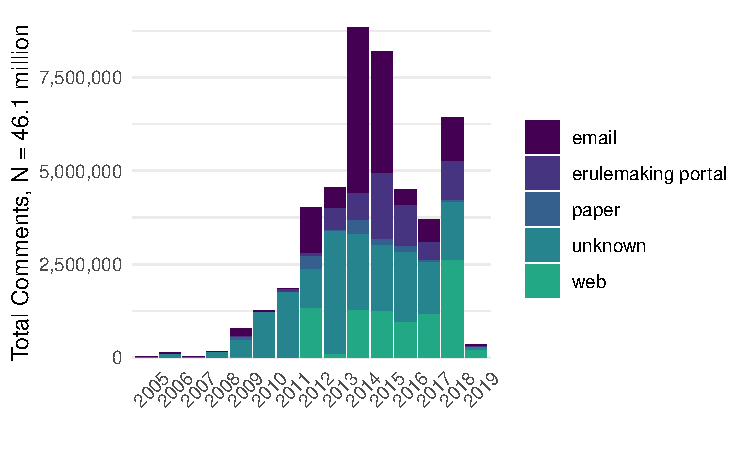
\includegraphics[width=6.5in]{../Figs/comments-from} 

}

\caption{Sources of Comments Posted to regulations.gov}\label{fig:comments-from}
\end{figure}

\begin{figure}[h!]
    \centering
        \caption{Rules in Order of Number of Comments}
    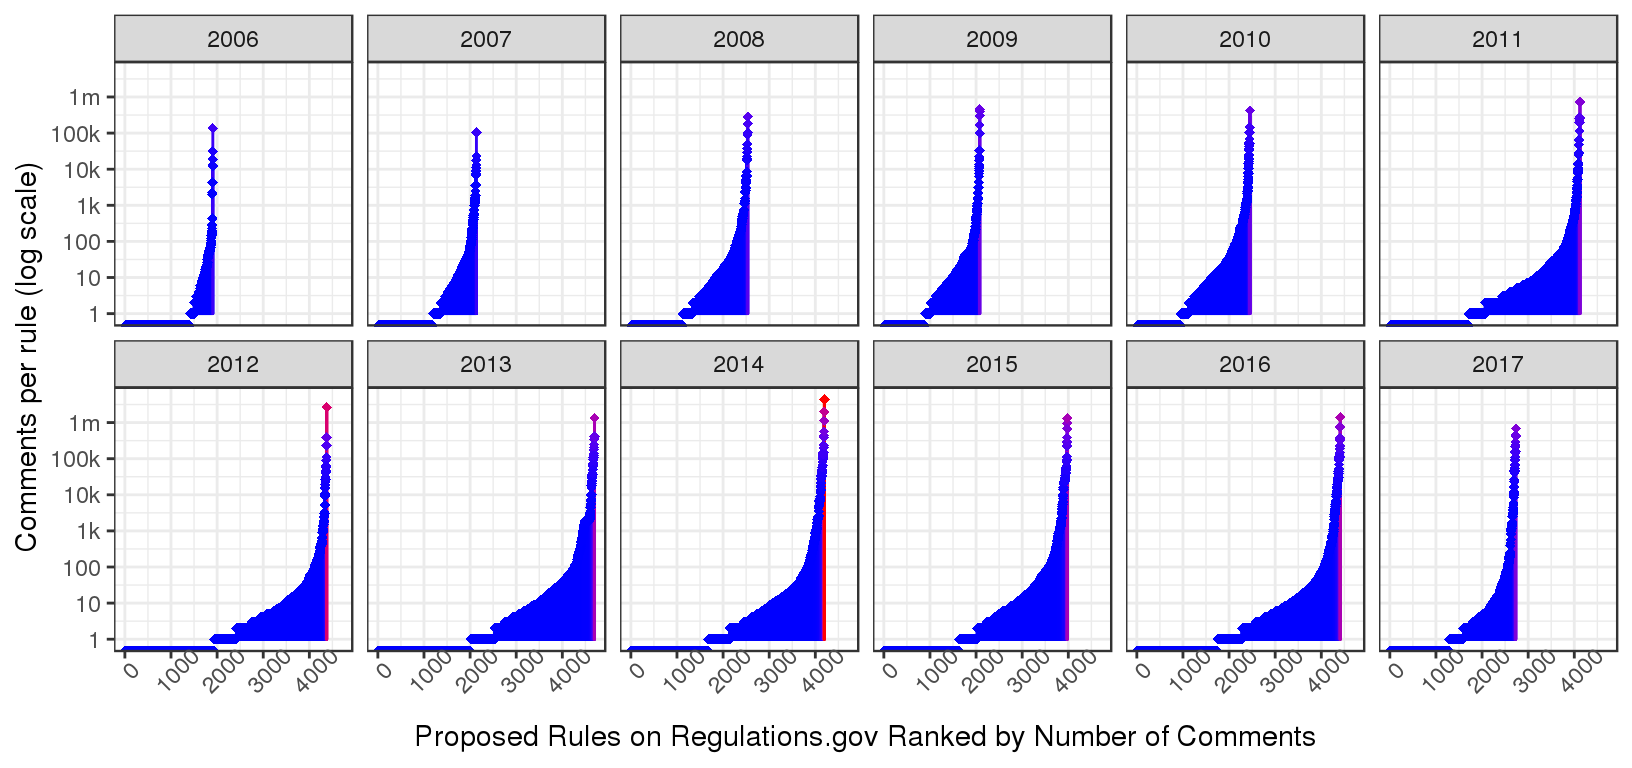
\includegraphics[width = 6.5in]{../Figs/rules-ranked-comments-per-year-1.png}
    \label{fig:rules-ranked}
\end{figure}

\begin{figure}[p!]
    \centering
        \caption{Major and Non-major Rules on regulations.gov}
    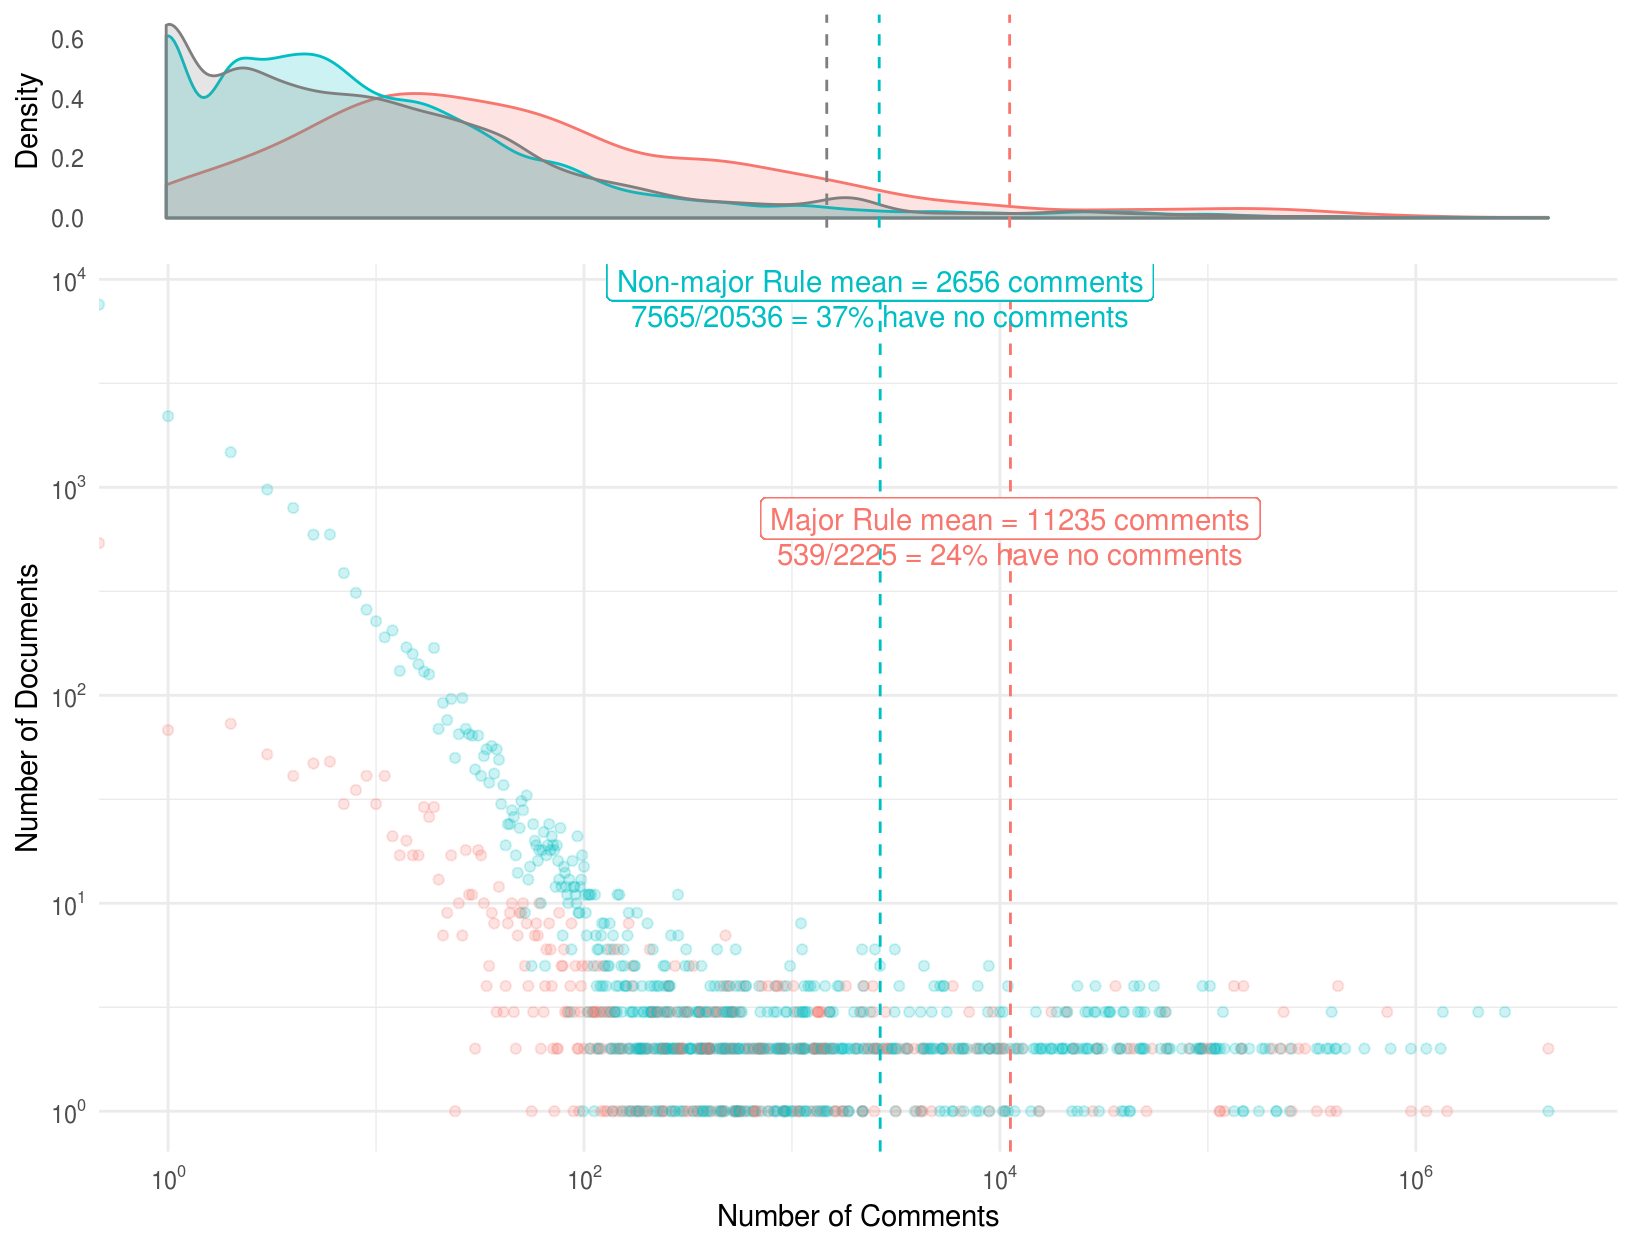
\includegraphics[width = 7in]{../Figs/major-comments-density-1.png}
    \label{fig:rules-major}
\end{figure}

\begin{figure}[p!]
    \centering
        \caption{Rules on regulations.gov by Unified Agenda Priority Level}
    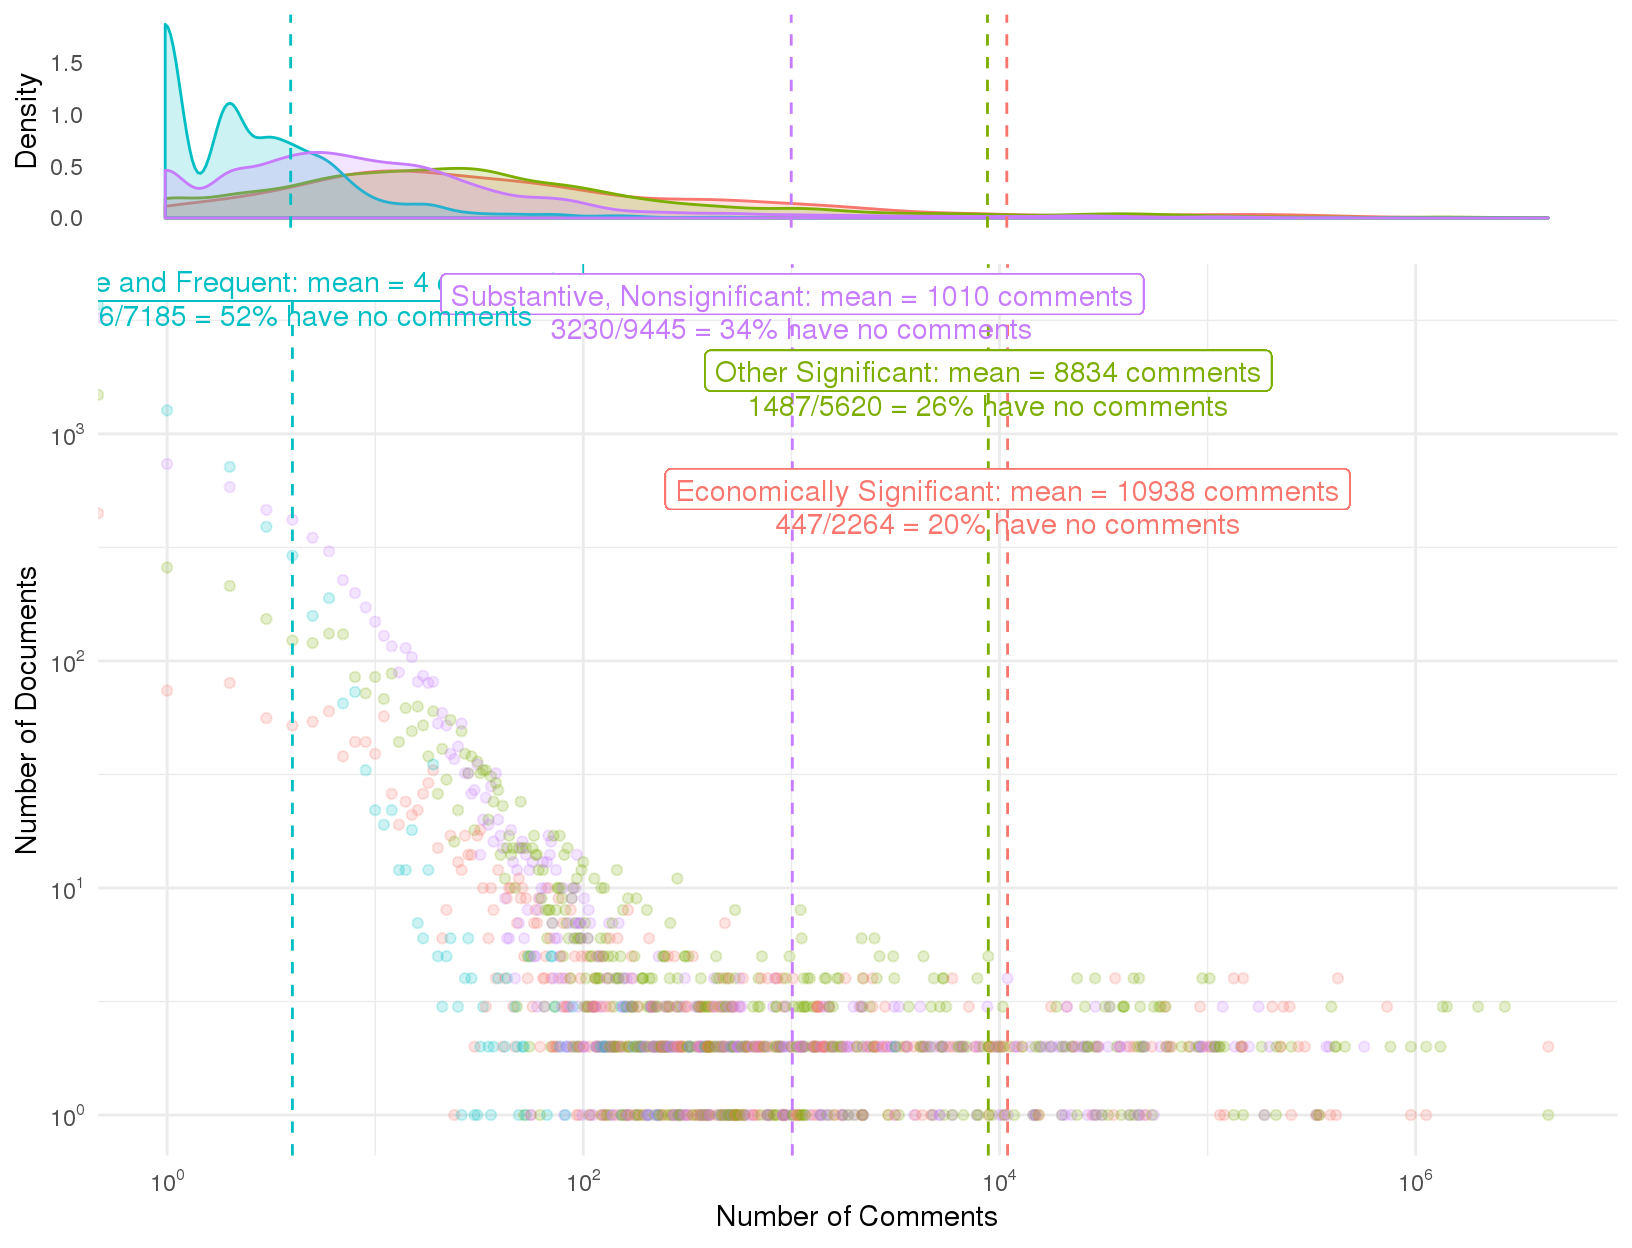
\includegraphics[width = 7in]{../Figs/priority-comment-density-1.png}
    \label{fig:rules-priority}
\end{figure}

\clearpage

\begin{figure}
    \caption{Unique or Partially Unique Comments by Sentiment Score (Sample of 2018 Rules)}
    \label{fig:sentiment-2018}
    \centering
    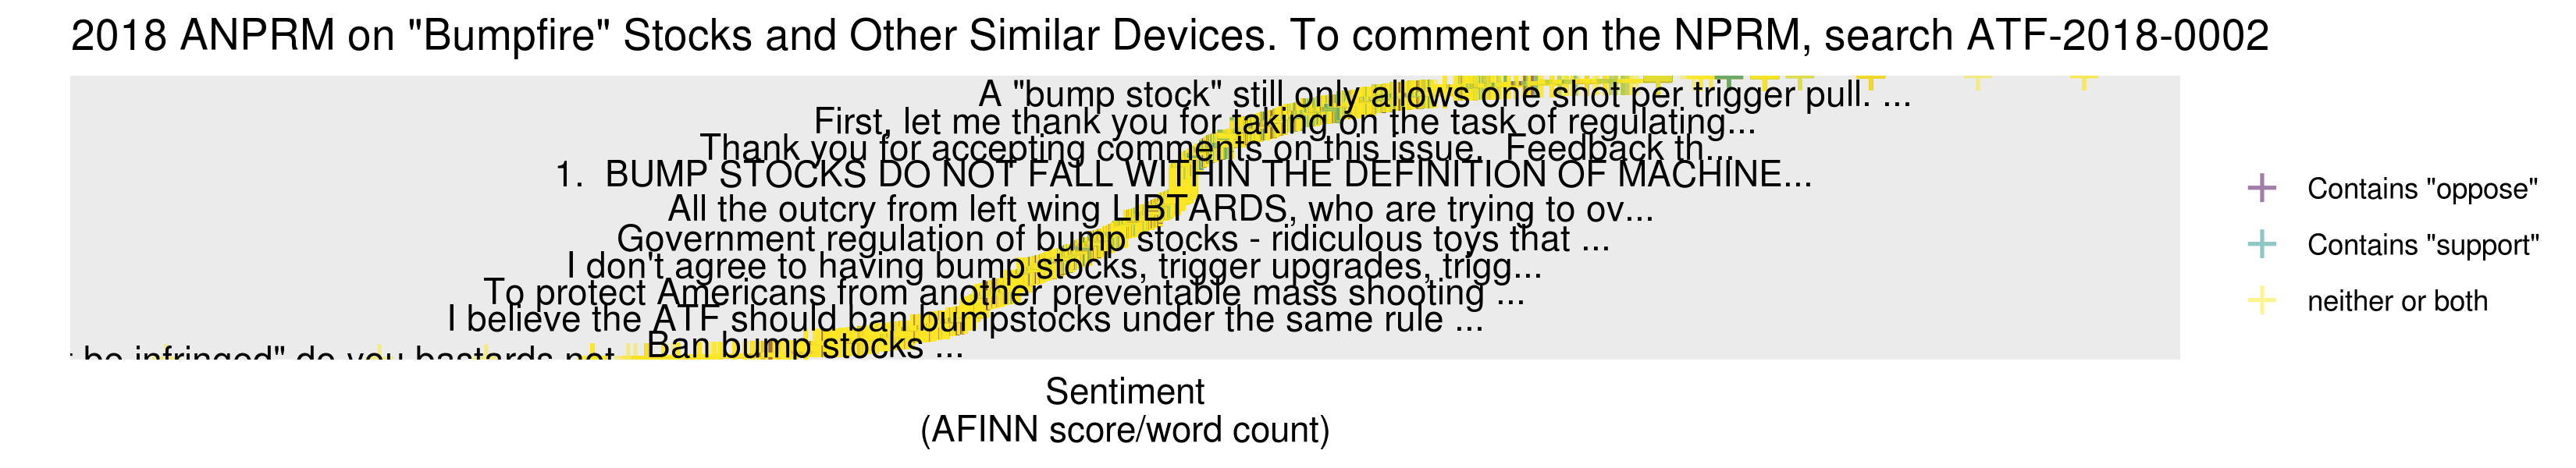
\includegraphics[width = 7in]{../Figs/sent-2018ATF-2018-0001.png}
    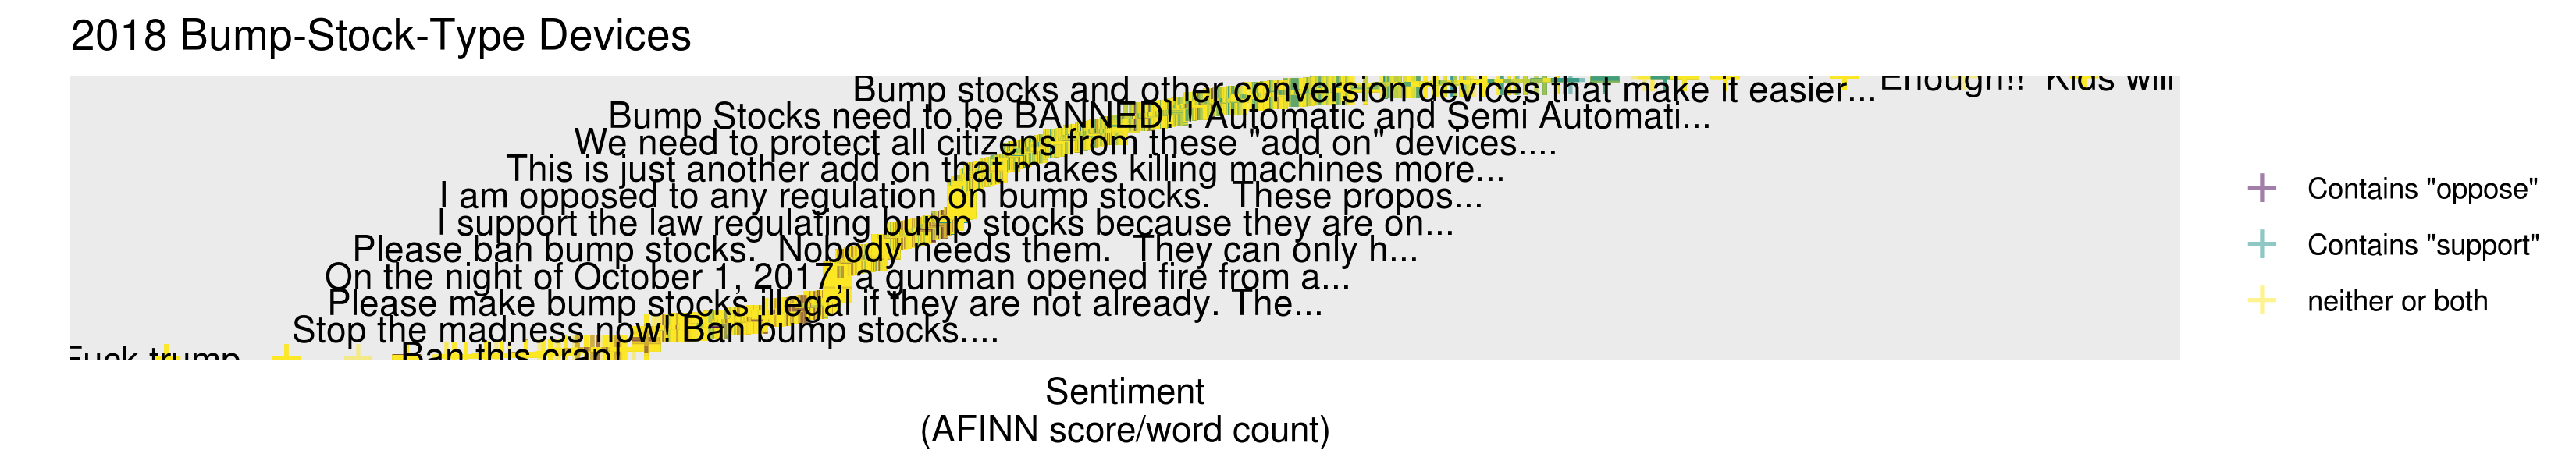
\includegraphics[width = 7in]{../Figs/sent-2018ATF-2018-0002.png}
    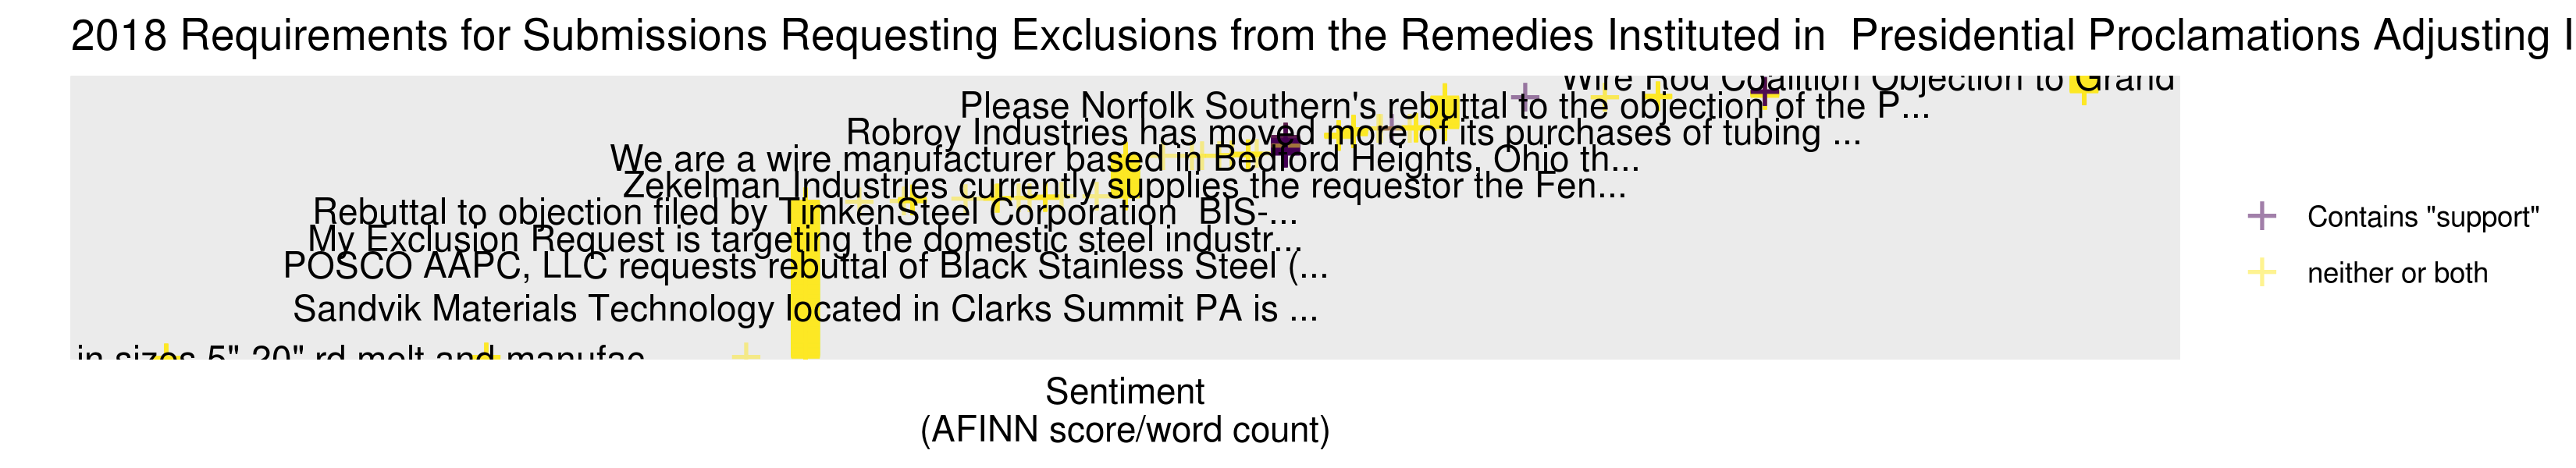
\includegraphics[width = 7in]{../Figs/sent-2018BIS-2018-0006.png}
    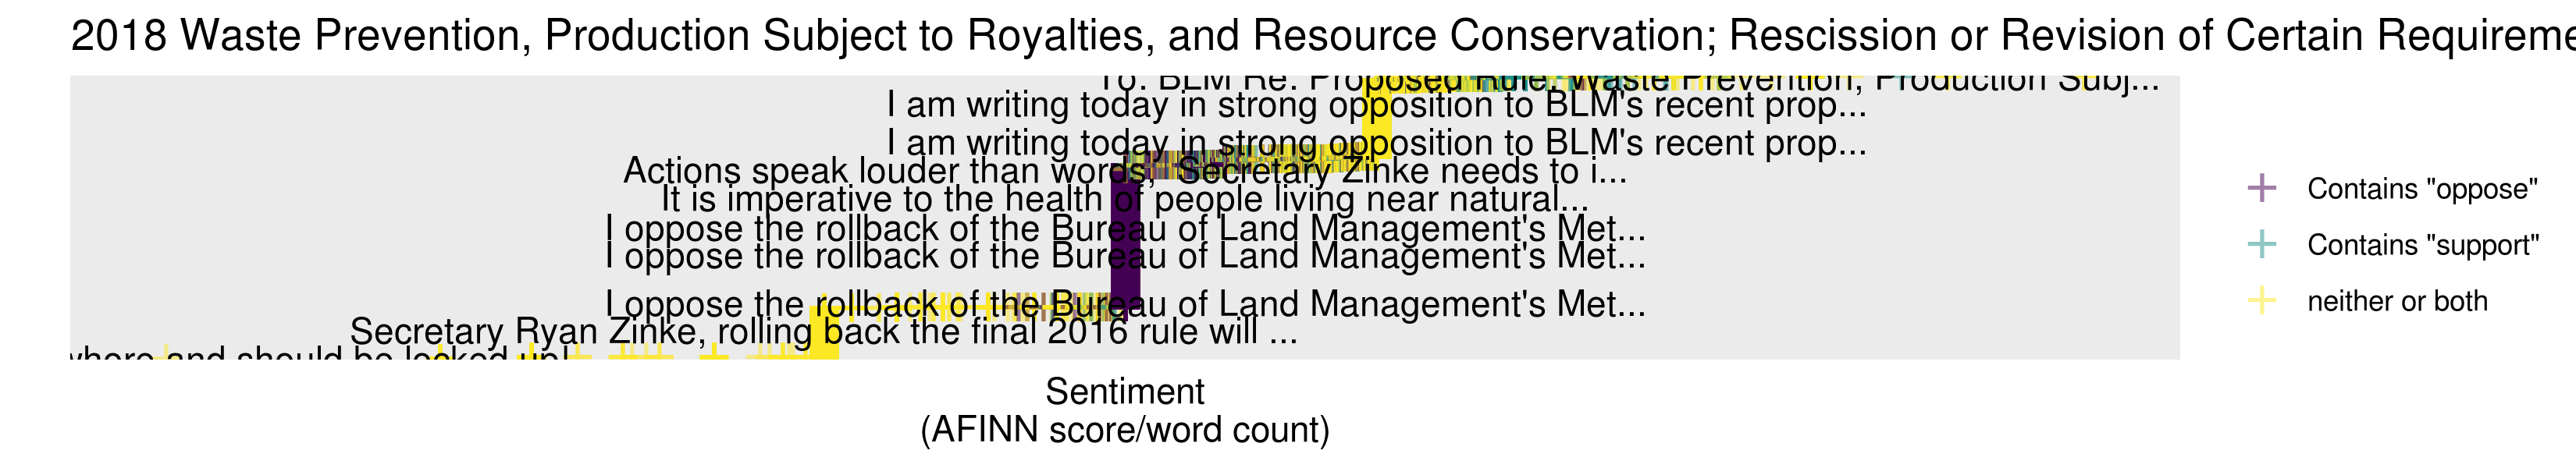
\includegraphics[width = 7in]{../Figs/sent-2018BLM-2018-0001.png}
    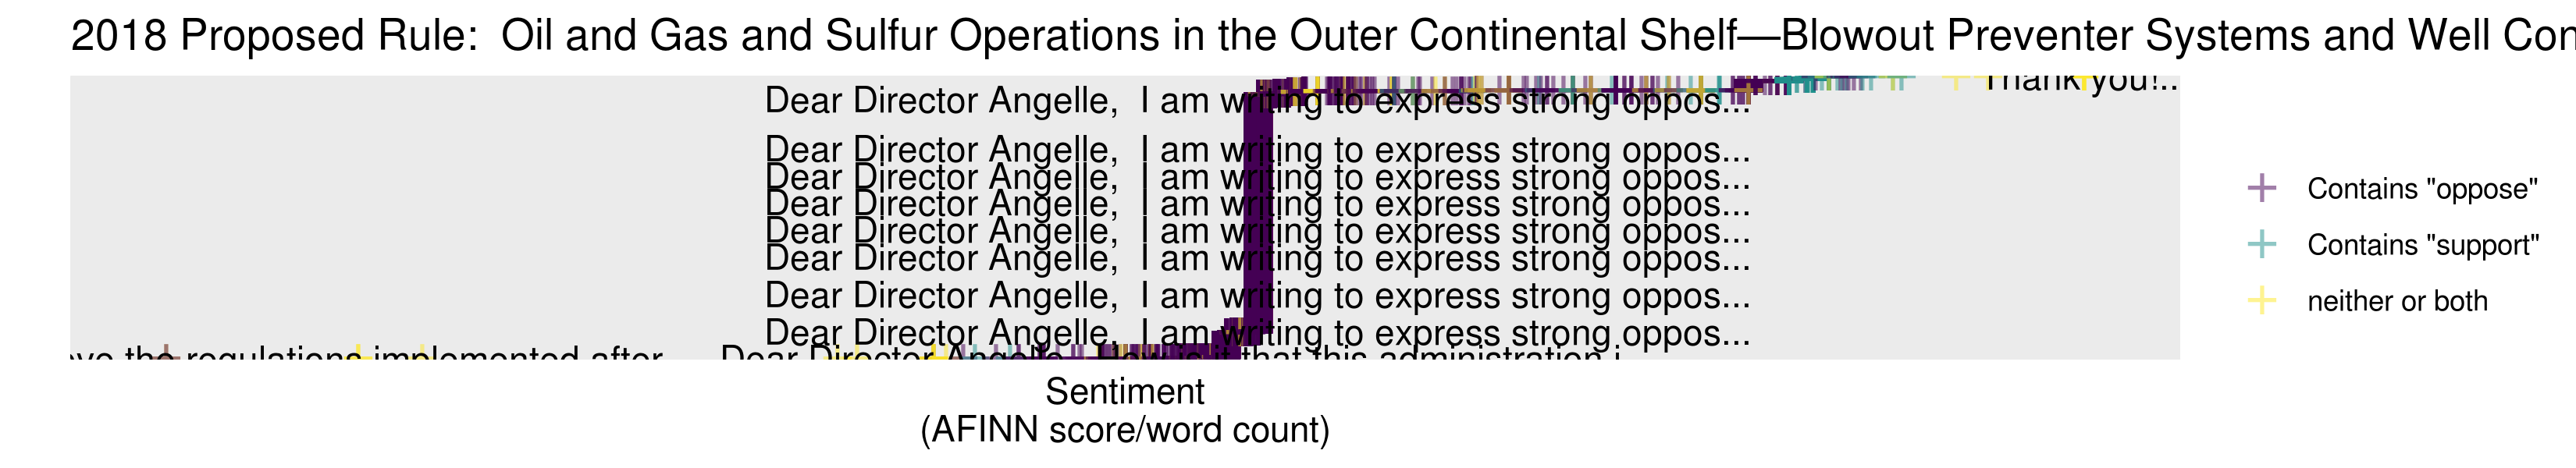
\includegraphics[width = 7in]{../Figs/sent-2018BSEE-2018-0002.png}
    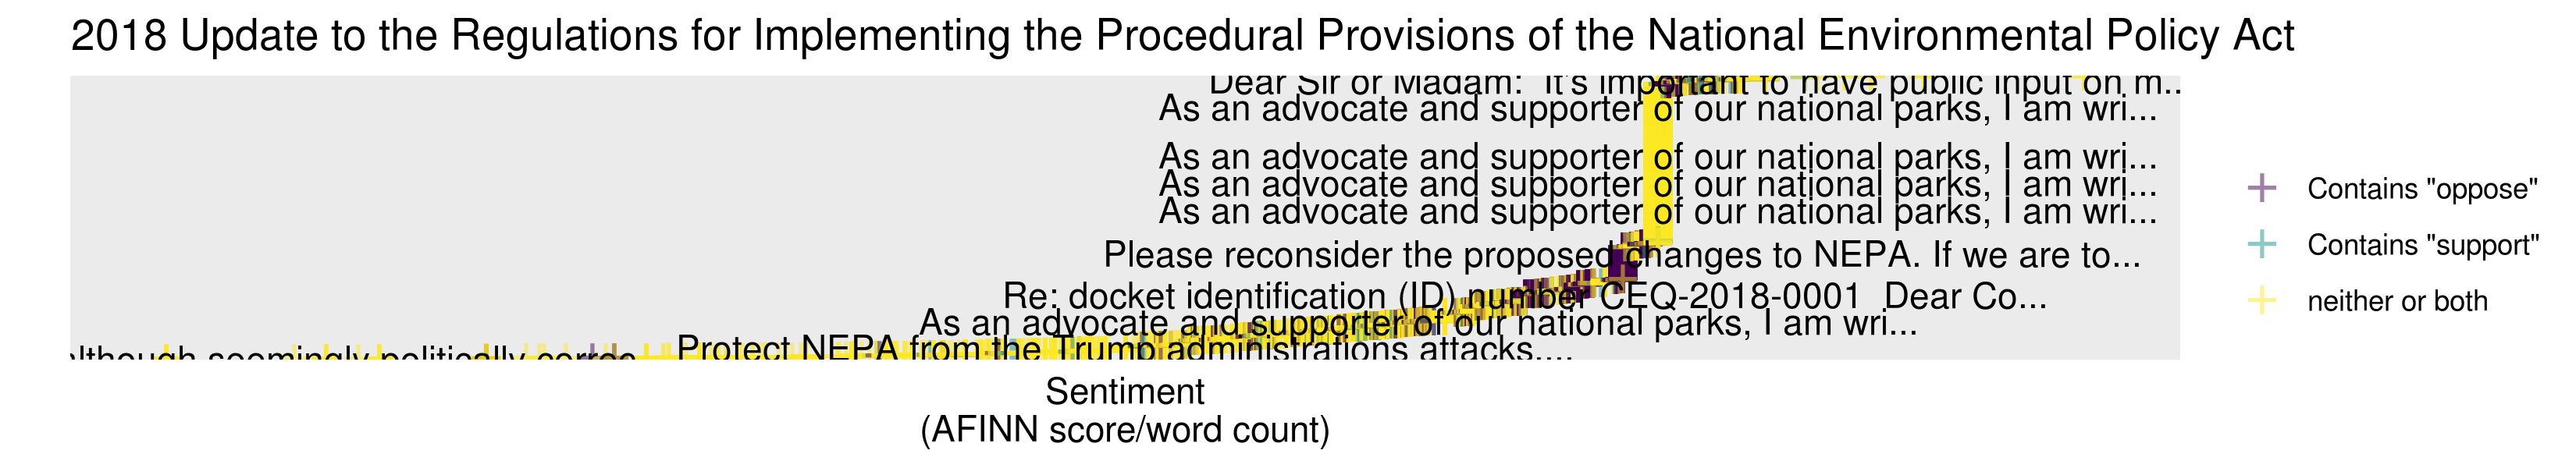
\includegraphics[width = 7in]{../Figs/sent-2018CEQ-2018-0001.png}
\end{figure}

\begin{figure}
    \caption{Unique or Partially Unique Comments by Sentiment Score (Sample of 2016 Rules)}
    \label{fig:sentiment-2016}
    \centering
    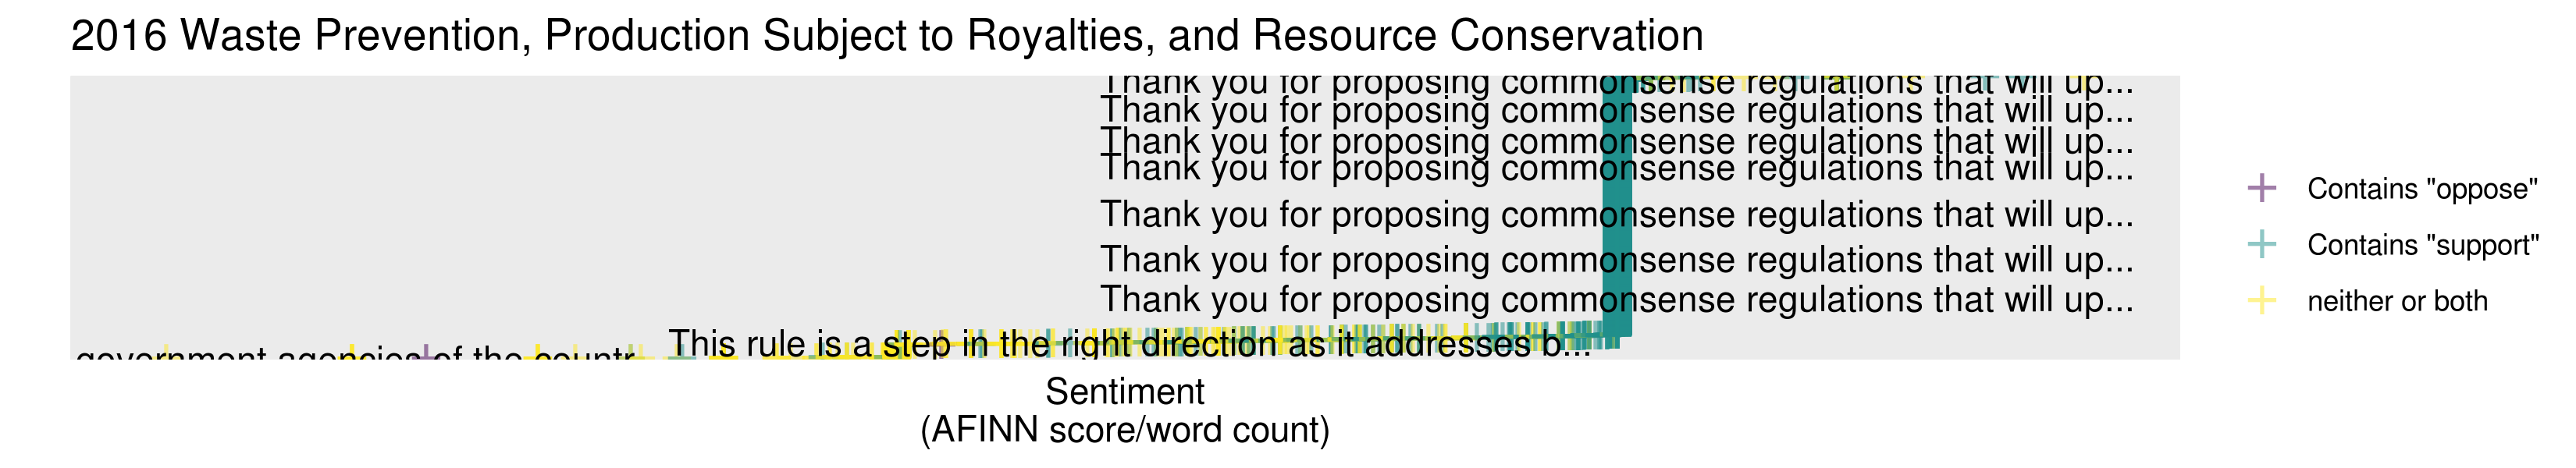
\includegraphics[width = 7in]{../Figs/sent-2016BLM-2016-0001.png}
    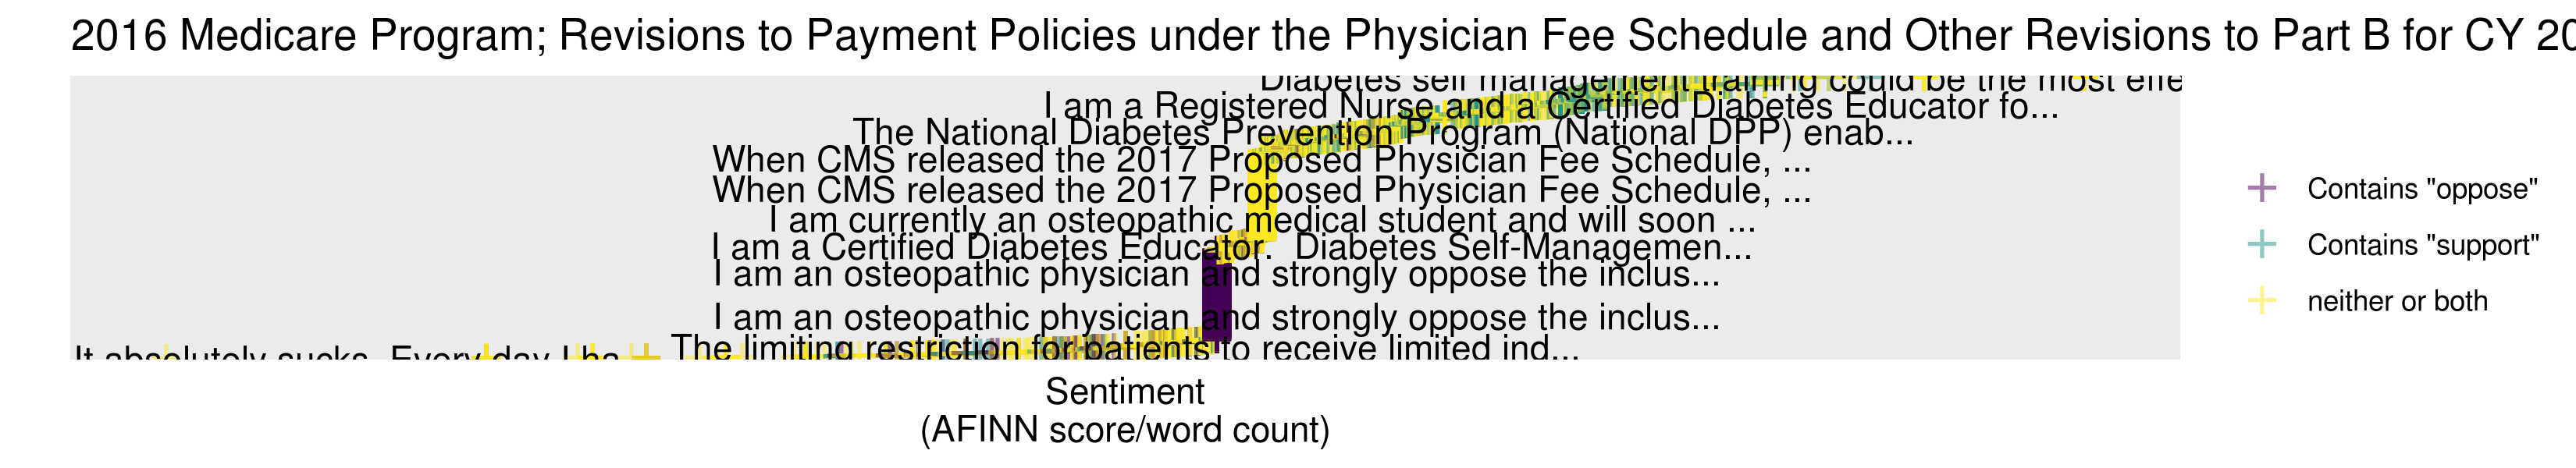
\includegraphics[width = 7in]{../Figs/sent-2016CMS-2016-0116.png}
    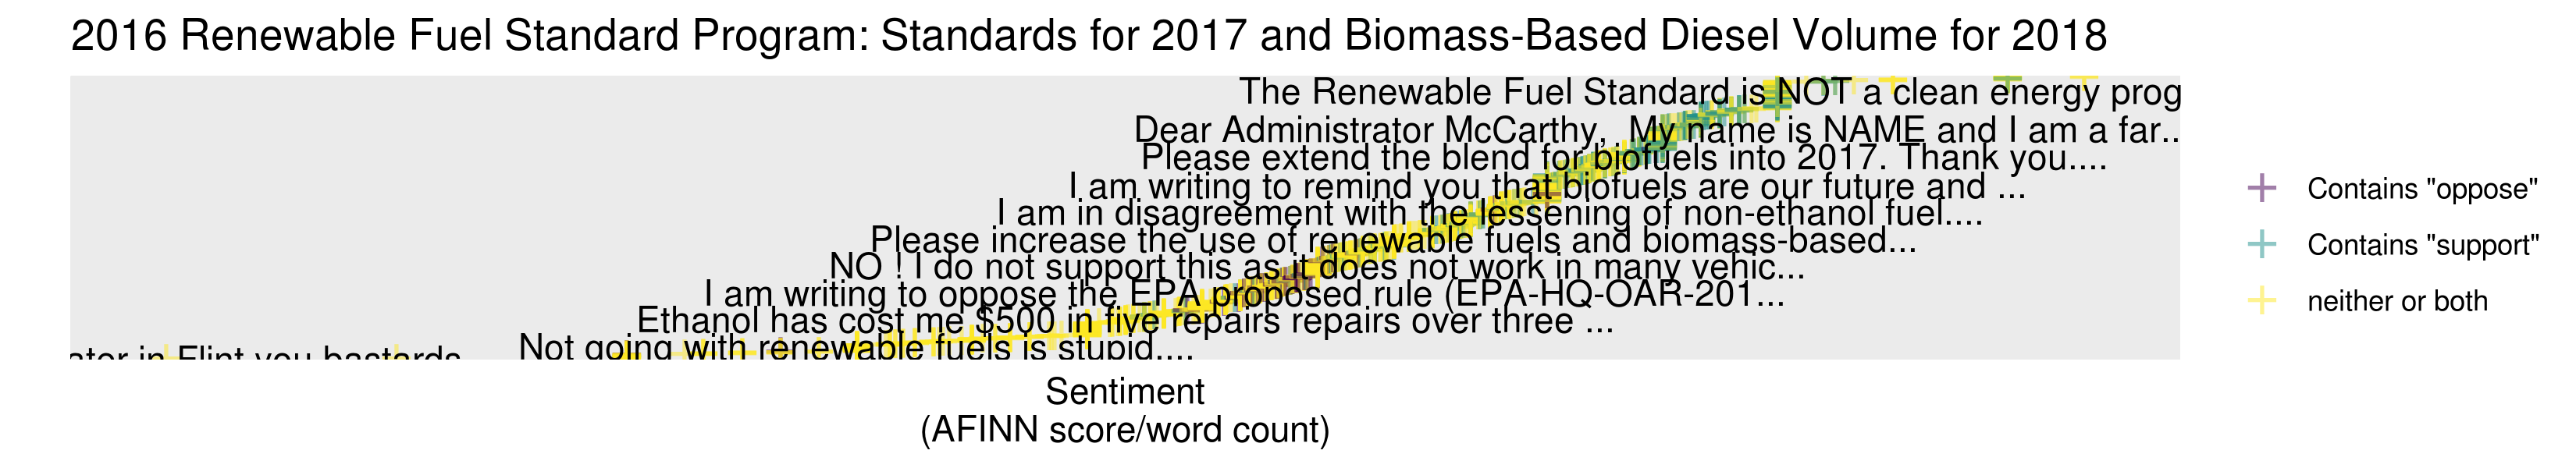
\includegraphics[width = 7in]{../Figs/sent-2016EPA-HQ-OAR-2016-0004.png}
    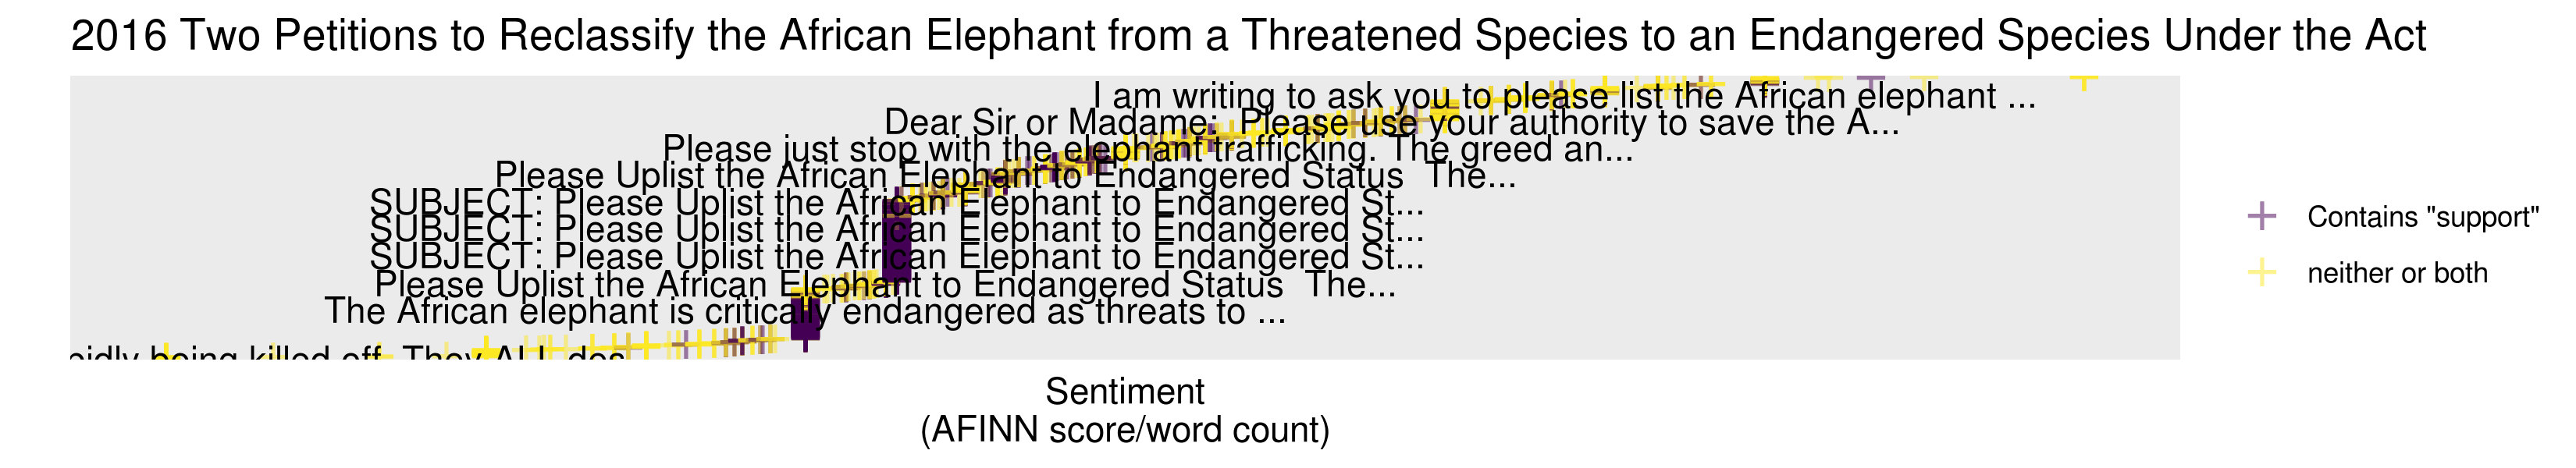
\includegraphics[width = 7in]{../Figs/sent-2016FWS-HQ-ES-2016-0010.png}
    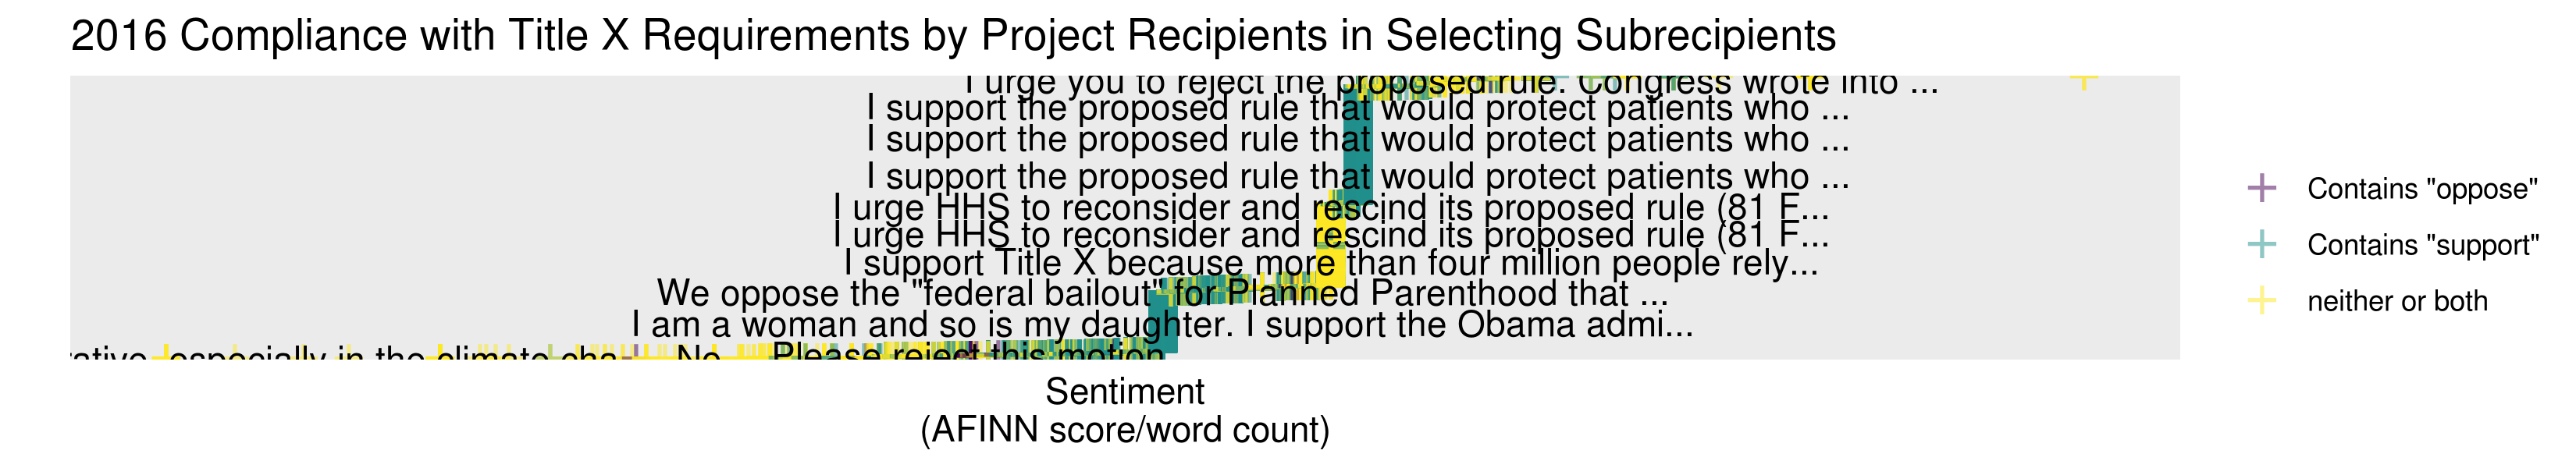
\includegraphics[width = 7in]{../Figs/sent-2016HHS-OS-2016-0014.png}
    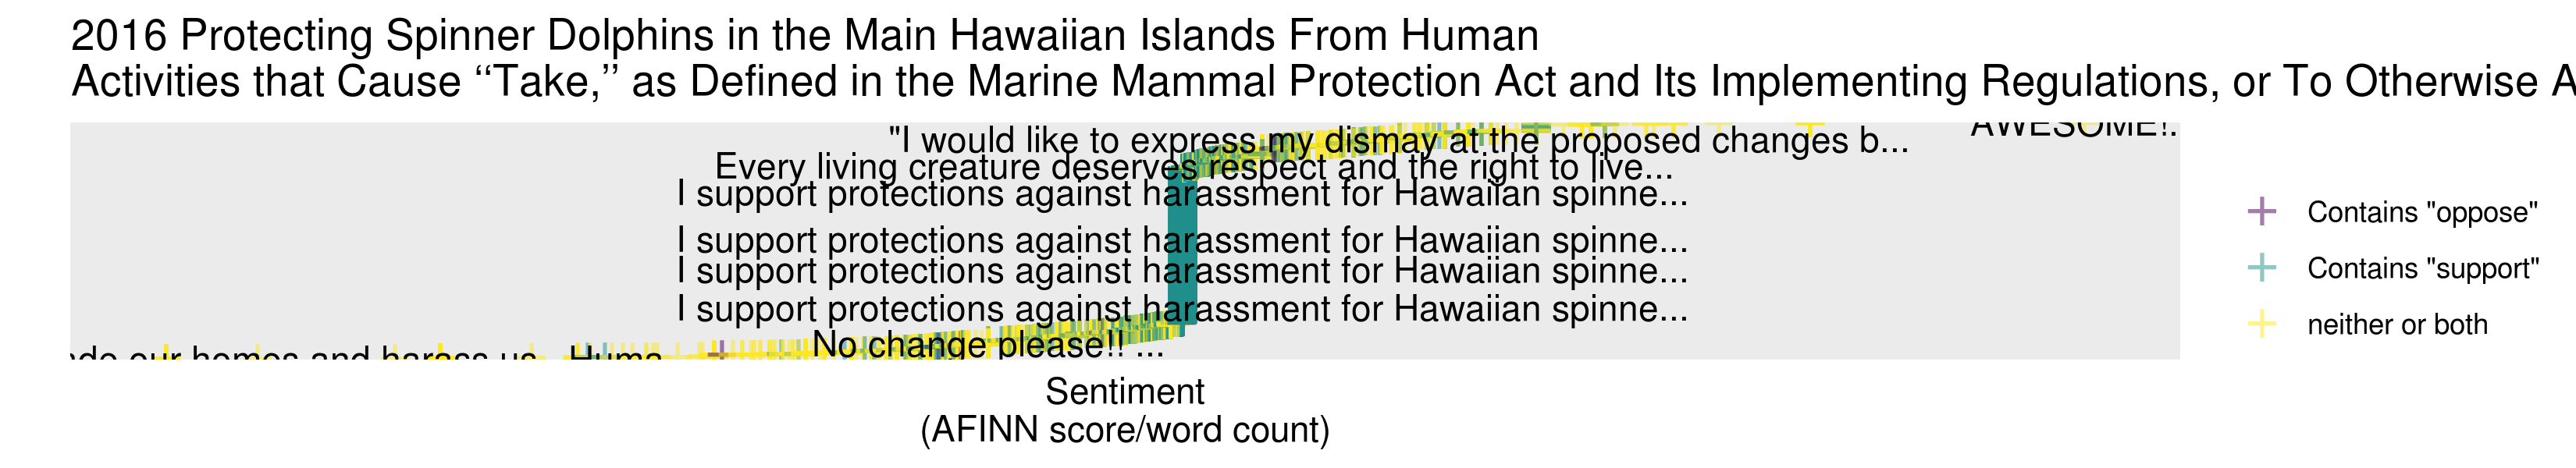
\includegraphics[width = 7in]{../Figs/sent-2016NOAA-2005-0226.png}
\end{figure}

\clearpage
% --- PAGE: endnotes -----------------------
% --- PAGE: refs -----------------------
\newpage
\singlespacing 
          \bibliography{/Users/devin/dissertation/assets/dissertation.bib} 
   

\end{document}
